\documentclass[11pt]{article}

\usepackage[margin=1in]{geometry}
\usepackage{amsmath,amssymb,mathtools}
\usepackage{graphicx}
\usepackage{hyperref}
\usepackage{booktabs}
\usepackage{caption}
\usepackage{subcaption}

\hypersetup{
    colorlinks=true,
    linkcolor=blue,
    urlcolor=blue,
    citecolor=blue
}

\newcommand{\Z}{\mathbb{Z}}
\newcommand{\R}{\mathbb{R}}
\newcommand{\N}{\mathbb{N}}
\newcommand{\T}{\mathbb{T}}

\title{On the Diophantine Stability of the Syracuse Map}

\author{John A.\ Janik\\
john.janik@gmail.com}
\date{\today}

\begin{document}
\maketitle

\begin{abstract}
We present the results of an exhaustive branch locus computation for
the Collatz map on the family of finite tori
$\T^2_k = (\Z/k\Z)^2$, carried out for all
$n \le 10^{11}$ across 27 hierarchically nested grid levels
($k \in \{1, 2, 3, \ldots, 19683\}$).  The computation consumed
61.5~hours on a 24-core Intel Core Ultra~9 275HX, accumulating
$25.1 \times 10^{12}$ Collatz steps.  Eight figures document the
principal findings: cell saturation, torus heatmaps, Diophantine
signatures, shift-of-finite-type (SFT) forbidden transitions,
foliation enrichment collapse, cell-level statistics, convergence
over~$N$, and transition/shadow analysis.  A comparison with the
earlier $10^{10}$ run reveals new structure invisible at lower~$N$:
a ``Diophantine ghost island'' of 251~cells at perpendicular
distance~370 from the main branch locus, created by the best rational
approximant $460/729 \approx \log_3 2$, together with a sharpened
gap in the shadow offset distribution and a new downward-sloping
feature in the foliation-position shadow profile.
\end{abstract}

%------------------------------------------------------------------
\section{Overview of the computation}
\label{sec:overview}

The \emph{branch locus} of the Collatz map at resolution~$k$ is the
set of cells $(r_2, r_3) \in (\Z/k\Z)^2$ that are visited by
trajectories with \emph{both} even and odd steps.  The complementary
cells---\emph{pure even} (only even steps land there) and
\emph{pure odd} (only odd steps)---carry deterministic parity and
are therefore confined to a single leaf of the Anosov-like foliation.

For each starting value $n = 1, 2, \ldots, 10^{11} - 1$, we iterate
the Collatz map $T(n) = n/2$ (if even) or $T(n) = 3n+1$ (if odd),
and at every step~$t$ we record the residue class
$(r_2, r_3) = (\nu_2(t) \bmod k,\; \nu_3(t) \bmod k)$ for each of the
27~grid levels $k = 3^a \cdot 2^b$ with $0 \le a,b$ and
$k \le 19{,}683$.  We also record transition types (even$\to$even,
even$\to$odd, etc.) and foliation/shadow geometry.

Key parameters:
\begin{center}
\begin{tabular}{ll}
\toprule
Total trajectories & $99{,}999{,}999{,}999$ \\
Total Collatz steps & $25{,}125{,}922{,}364{,}266$ \\
Mean trajectory length & $251.26$ steps \\
Global $p_{\mathrm{odd}}$ & $0.332473361$ \\
Number of $k$-levels & 27 \\
Saturated branch cell count & $21{,}632$ (from $k = 216$ onward) \\
Runtime & 61.5~hours (24-thread OpenMP) \\
\bottomrule
\end{tabular}
\end{center}

%------------------------------------------------------------------
\section{Figure 1: Cell saturation and scale overview}
\label{sec:fig1}

\begin{figure}[htbp]
\centering
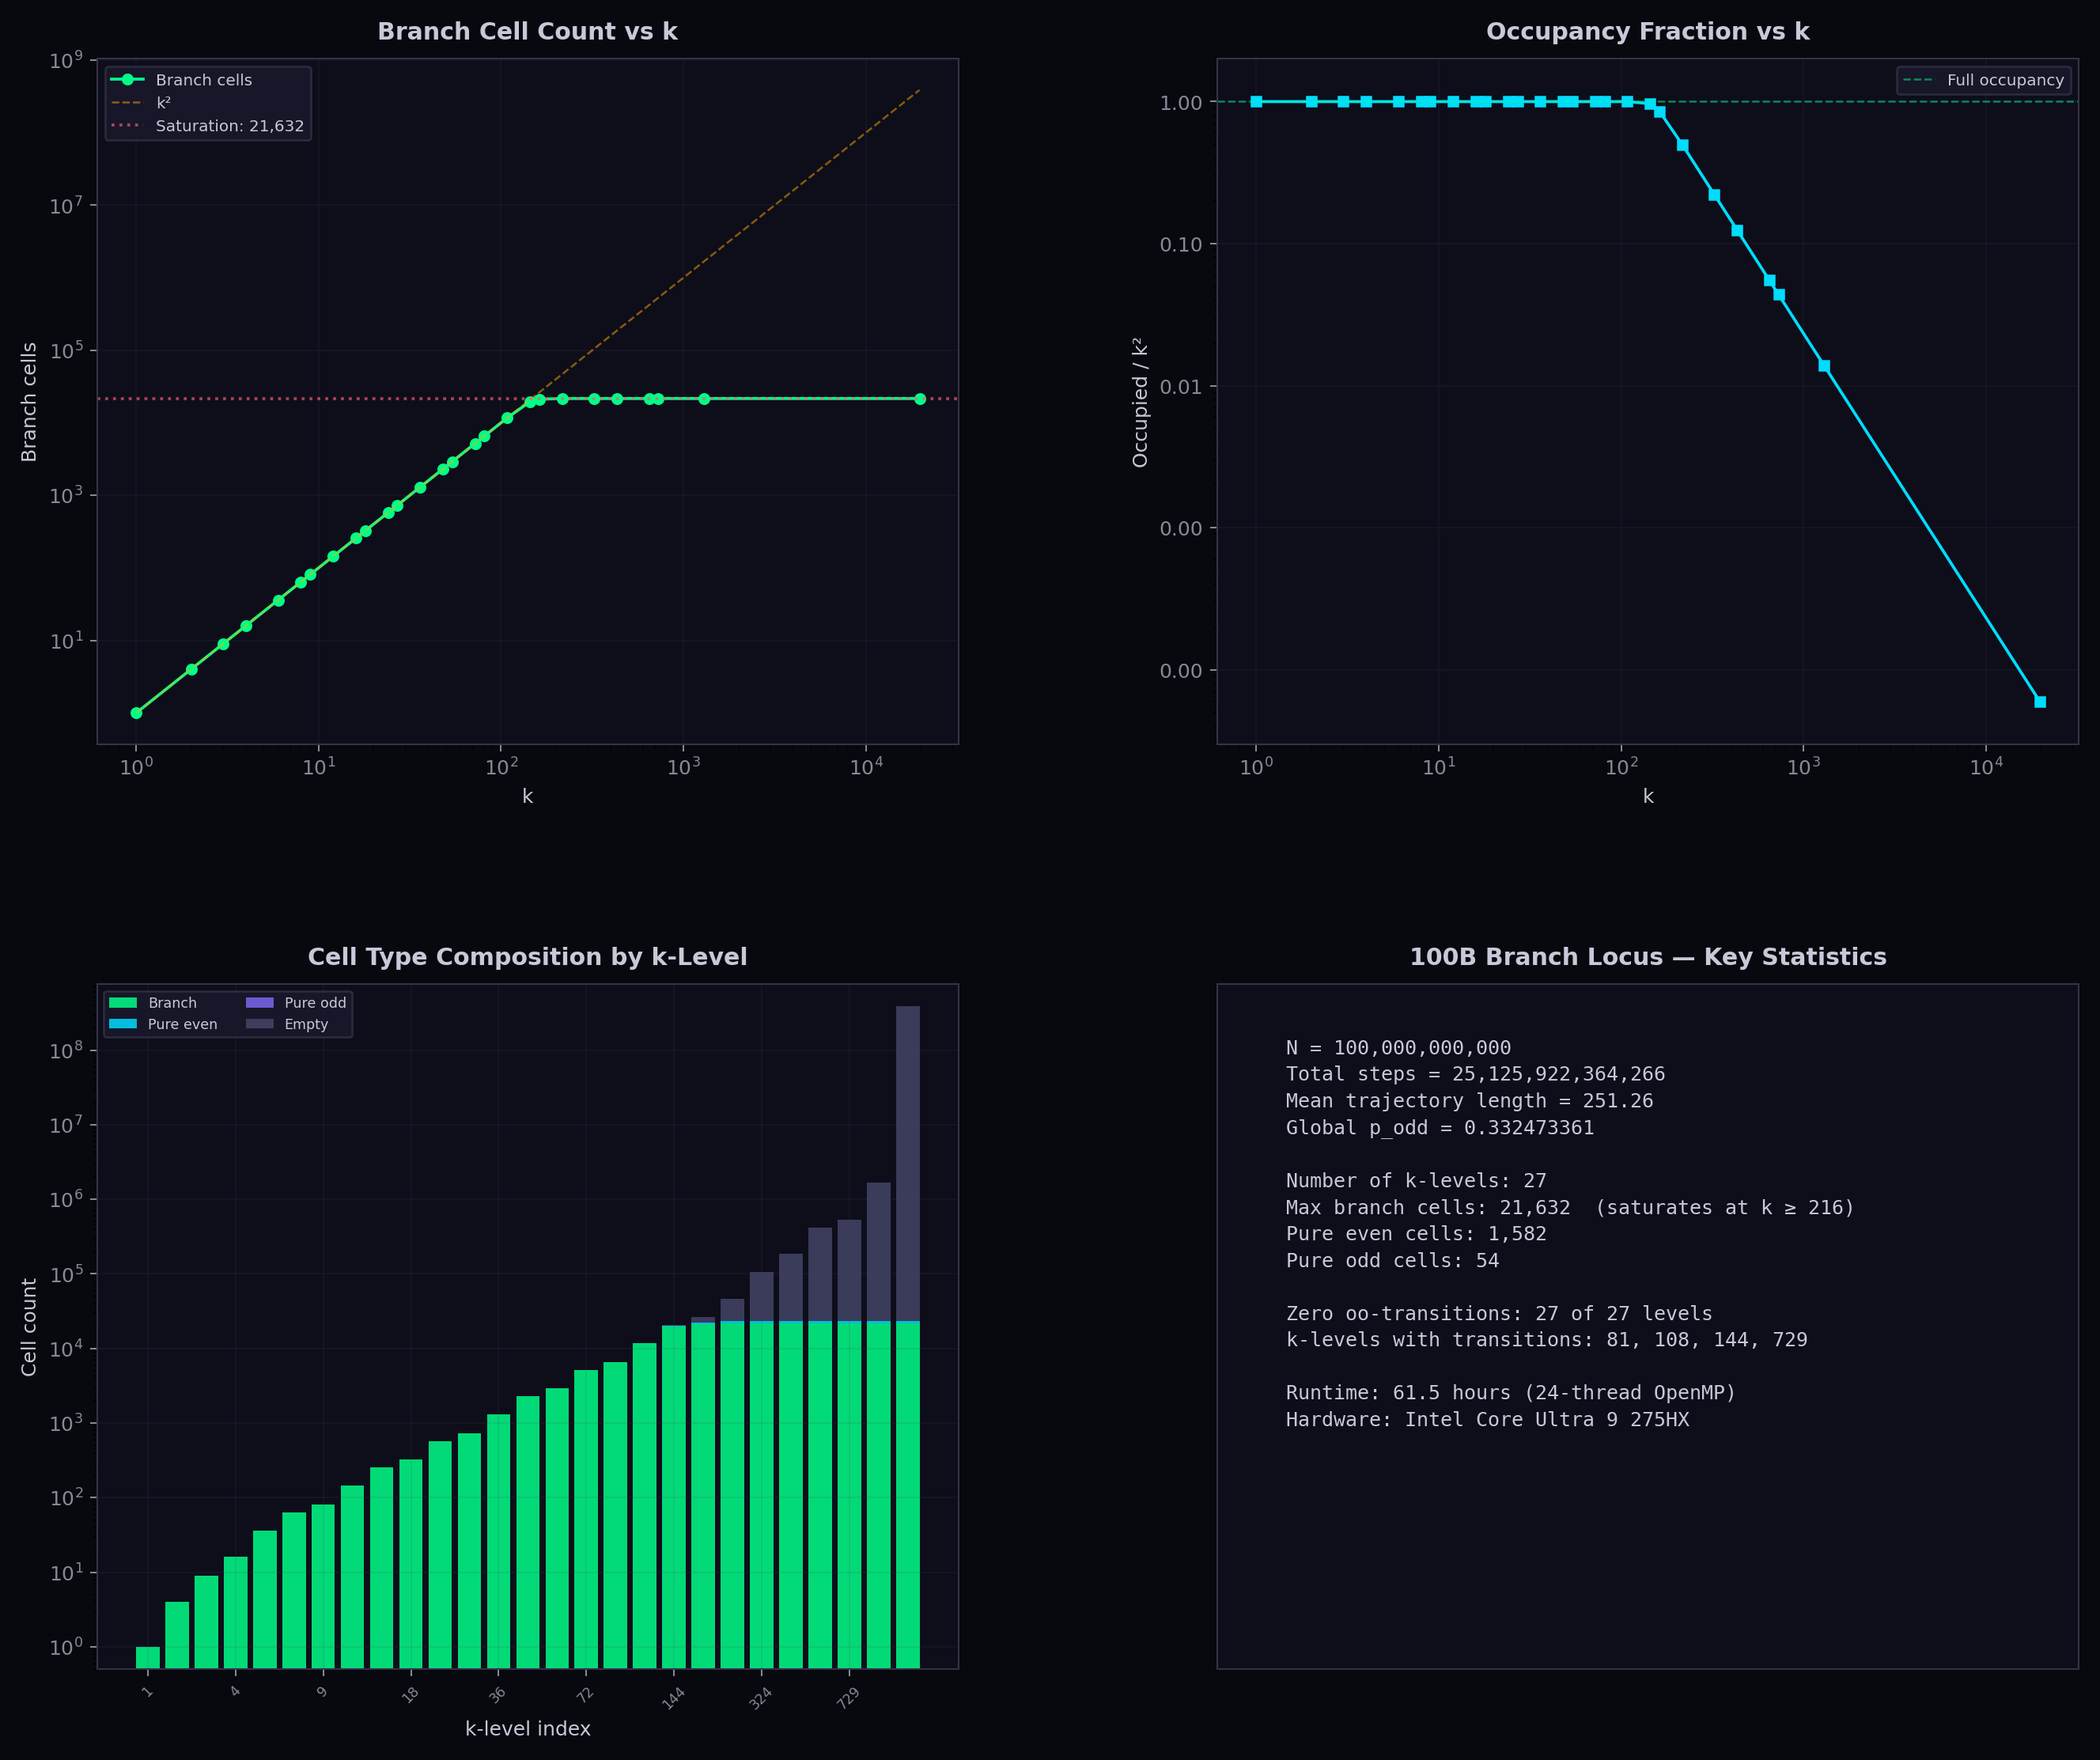
\includegraphics[width=\textwidth]{../visualizations/branch_locus_fig1.png}
\caption{Cell saturation and scale overview. \textbf{(a)}~Branch cell
  count vs.\ $k$ on log--log axes.  At small~$k$ every cell is
  branch (count $= k^2$); by $k = 216$ the count saturates at
  $21{,}632$ and remains frozen through $k = 19{,}683$.  The $k^2$
  reference line shows the departure from full occupancy.
  \textbf{(b)}~Occupancy fraction (occupied$/k^2$) drops from 1.0 at
  $k \le 108$ to $0.006\%$ at $k = 19{,}683$, meaning the vast
  majority of cells at high resolution are empty.
  \textbf{(c)}~Stacked cell-type composition across all 27~levels:
  branch (green), pure even (cyan), pure odd (purple), and empty
  (gray).  The transition from all-branch to predominantly-empty
  occurs between $k = 108$ and $k = 216$.  \textbf{(d)}~Key
  statistics panel summarizing the run.}
\label{fig:saturation}
\end{figure}

The saturation of branch cells at exactly $21{,}632$ is the central
empirical fact.  It means the torus $\T^2_k$ for $k \ge 216$ contains
a \emph{fixed} set of $21{,}632$ cells that carry all the dynamical
complexity.  The remaining $k^2 - 21{,}632$ cells are either
permanently empty or confined to a single parity.  This is consistent
with the Diophantine confinement picture: the irrational foliation
$r_3 = \log_2 3 \cdot r_2$ carves out a thin neighborhood that
captures all branch dynamics, while cells far from the foliation are
``repelled'' to pure-parity or emptiness.

The $1{,}582$ pure-even cells and $54$ pure-odd cells that appear at
$k \ge 216$ are arithmetically special: they correspond to residue
classes where the modular constraint forces a single parity choice.

%------------------------------------------------------------------
\section{Figure 2: Torus heatmaps at four scales}
\label{sec:fig2}

\begin{figure}[htbp]
\centering
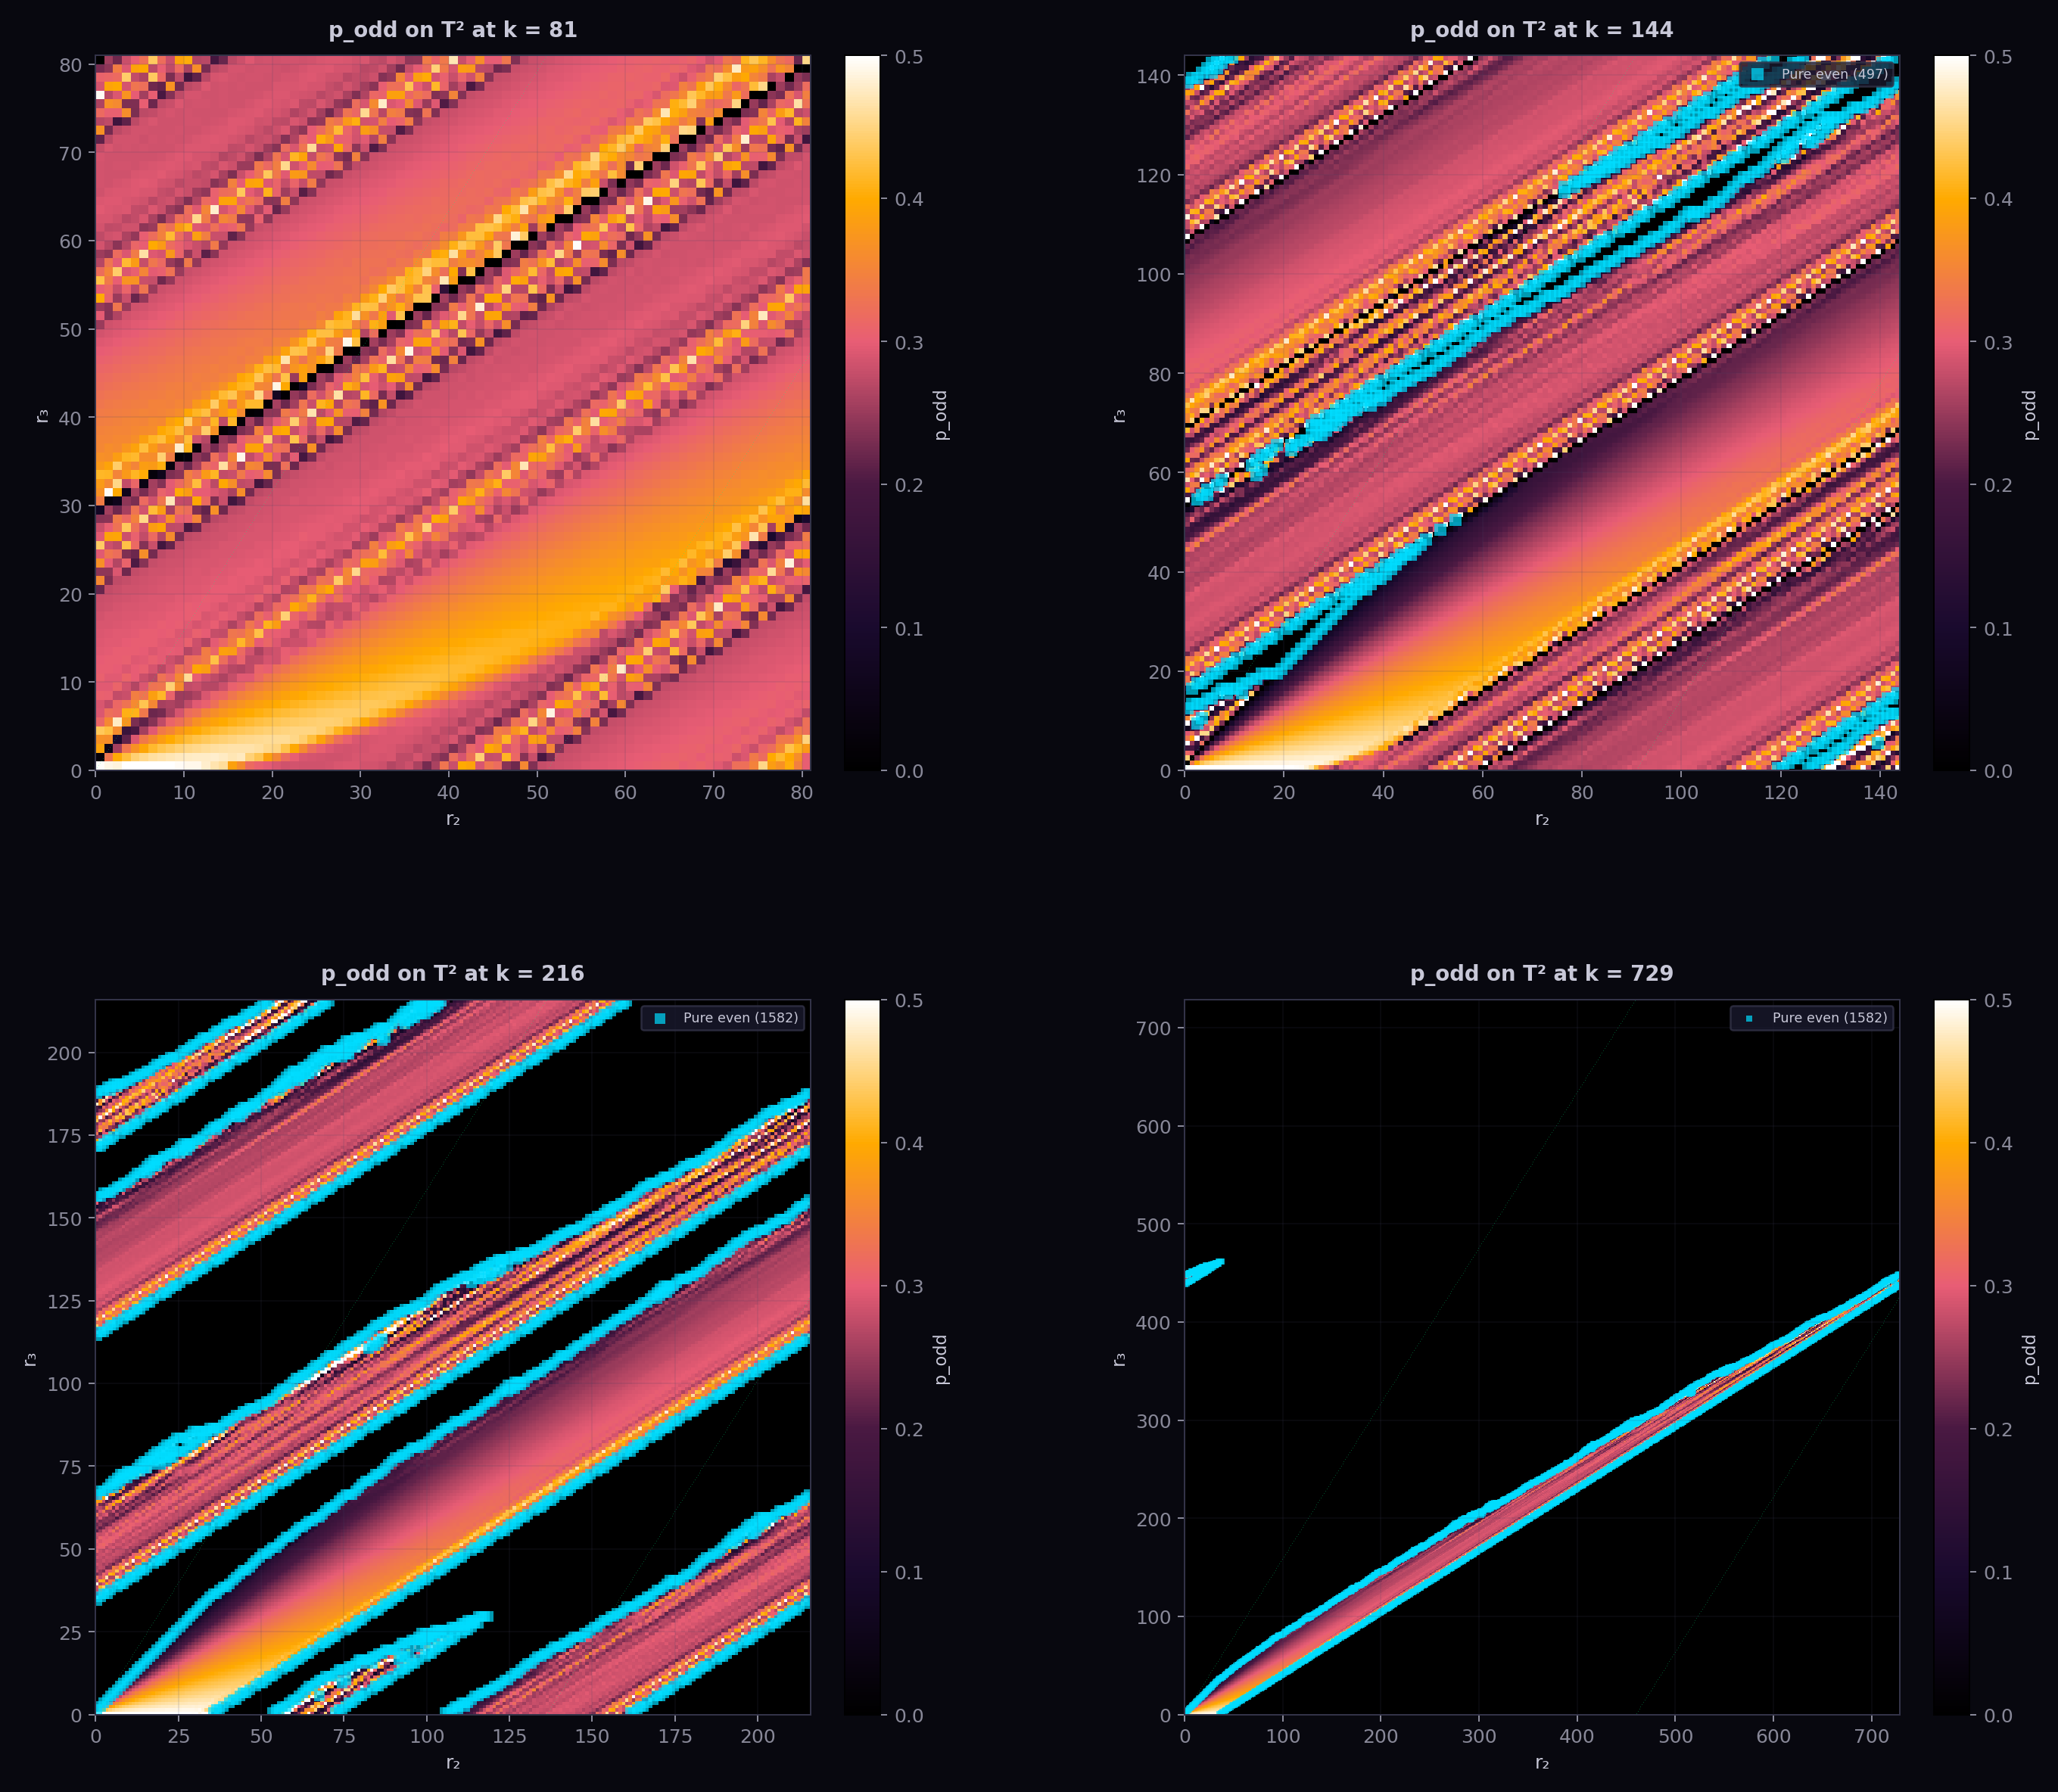
\includegraphics[width=\textwidth]{../visualizations/branch_locus_fig2.png}
\caption{Torus heatmaps of $p_{\mathrm{odd}}$ at four resolutions.
  Each pixel represents a cell $(r_2, r_3)$; color encodes the
  fraction of odd steps landing in that cell.  The green dots trace
  the irrational foliation $r_3 = \log_2 3 \cdot r_2 \pmod{k}$;
  cyan markers indicate pure-even cells.  \textbf{(a)}~$k = 81$:
  fully occupied, smooth gradient.  \textbf{(b)}~$k = 144$: first
  appearance of empty cells and pure-parity specialization.
  \textbf{(c)}~$k = 216$: transition complete, fractal-like
  occupancy pattern.  \textbf{(d)}~$k = 729$: sparse torus with
  only $\sim 4\%$ occupancy, branch cells concentrated near the
  irrational foliation.}
\label{fig:heatmaps}
\end{figure}

These heatmaps reveal the geometric structure of the branch locus
on the two-dimensional torus.  At $k = 81$, every cell is a branch
cell and $p_{\mathrm{odd}}$ varies smoothly, with the irrational
foliation passing through regions of moderate $p_{\mathrm{odd}}$.
By $k = 144$, the first empty cells appear along with pure-even
cells, which cluster near the foliation but on specific arithmetic
sublattices.  At $k = 729$, the torus is almost entirely dark
(empty), with occupied cells forming a fractal dust concentrated
near---but not exactly on---the irrational line.

The visual progression from smooth to fractal mirrors the algebraic
transition from a fully ergodic system (all residues visited) to a
Diophantine-constrained one where only cells within
$O(1/k)$ of the foliation survive.

%------------------------------------------------------------------
\section{Figure 3: Diophantine signature}
\label{sec:fig3}

\begin{figure}[htbp]
\centering
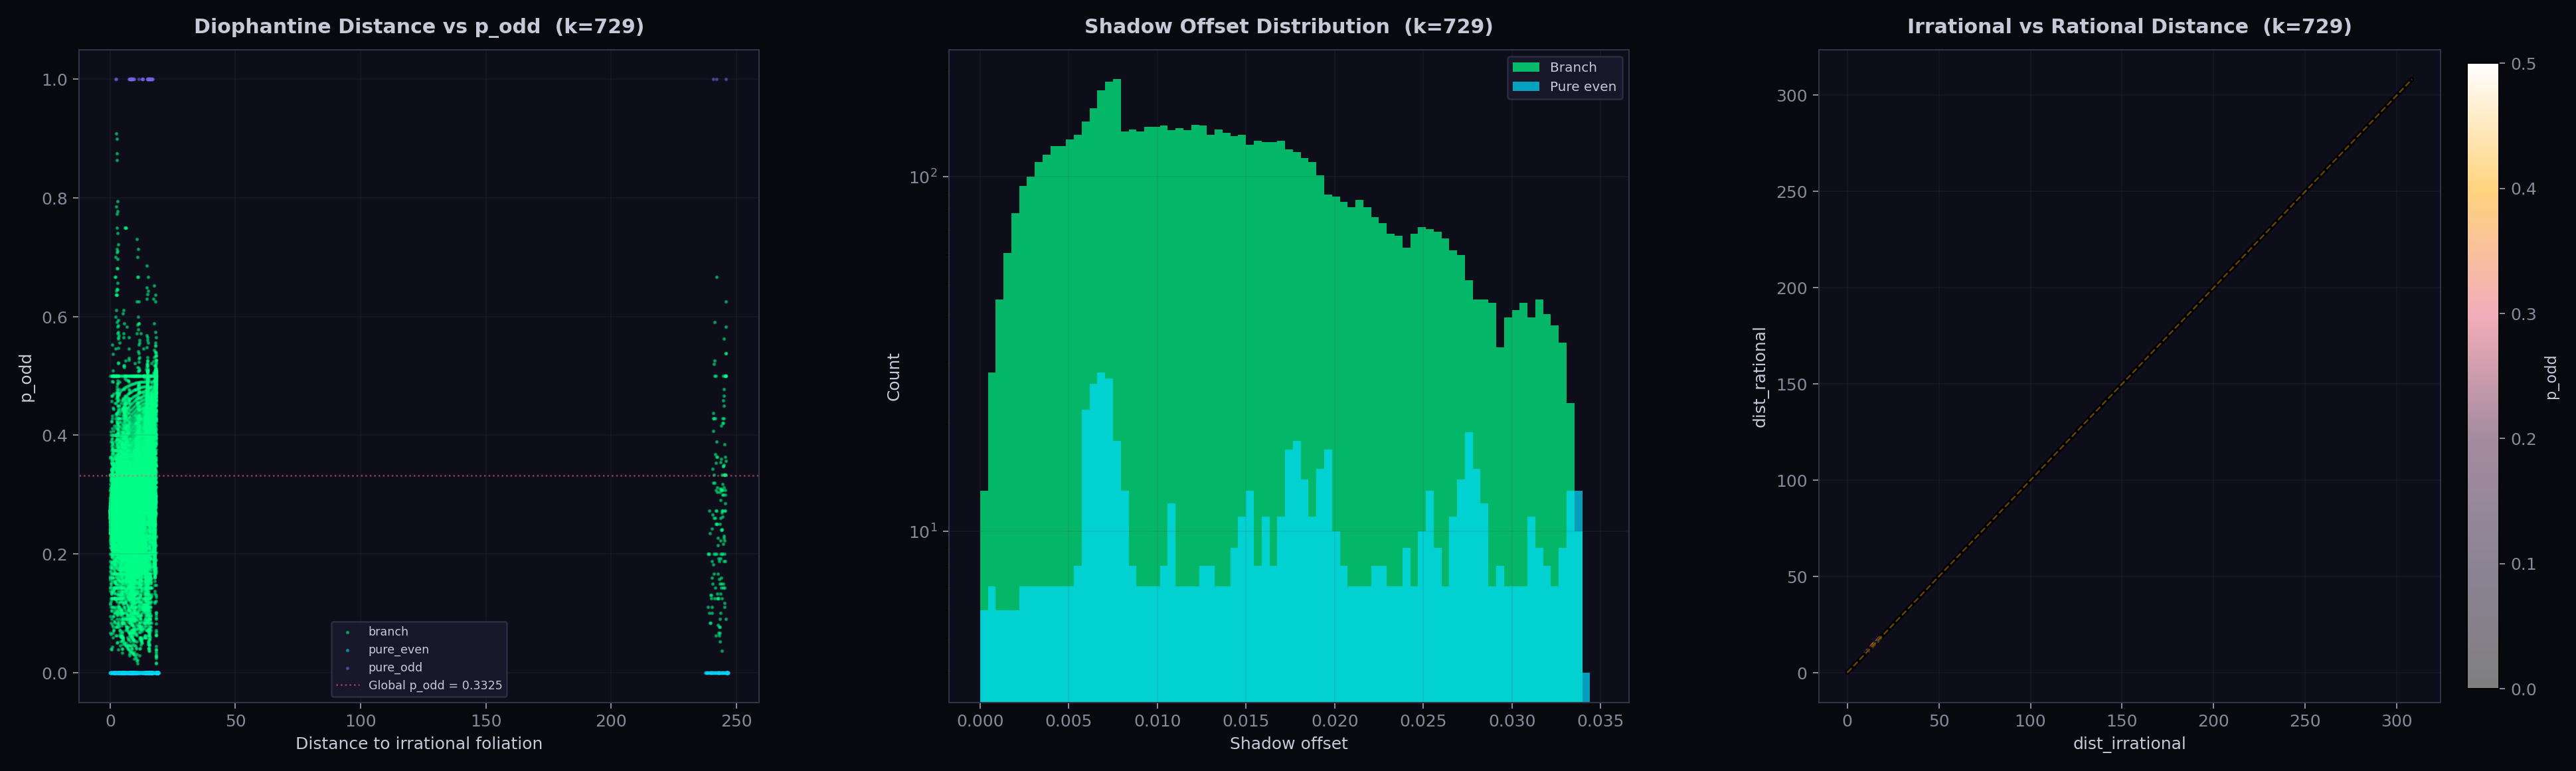
\includegraphics[width=\textwidth]{../visualizations/branch_locus_fig3.png}
\caption{Diophantine signature at $k = 729$.
  \textbf{(a)}~Distance to the irrational foliation vs.\ $p_{\mathrm{odd}}$,
  colored by cell type.  Branch cells (green) span a range of
  foliation distances and $p_{\mathrm{odd}}$ values.  Pure-even
  cells (cyan) cluster at $p_{\mathrm{odd}} = 0$ and moderate
  foliation distance.
  \textbf{(b)}~Shadow offset histogram: the gap between each cell's
  irrational and rational foliation distances.  Branch cells show a
  smooth distribution; pure-even cells are concentrated at specific
  offsets.
  \textbf{(c)}~Irrational vs.\ rational foliation distance, colored
  by~$p_{\mathrm{odd}}$.  Cells near the diagonal have comparable
  distances to both foliations; those far from the diagonal are
  ``captured'' by one foliation.}
\label{fig:diophantine}
\end{figure}

The Diophantine signature quantifies the relationship between each
cell's proximity to the irrational foliation
($r_3/r_2 \approx \log_2 3$) and its dynamical character.  The
\emph{shadow offset}---the gap between a cell's irrational and
rational foliation distances---measures how strongly the cell is
``pulled'' toward one foliation leaf versus the other.

Panel~(a) shows that branch cells span a continuous range of
foliation distances, while pure-even cells are confined to a narrow
band.  This is consistent with Baker's theorem: cells where the
rational approximation to $\log_2 3$ is too close (relative to the
Diophantine threshold $|p/q - \log_2 3| > c/q^\mu$) are forced into
pure parity.

Panel~(c) reveals a striking structure: cells with high
$p_{\mathrm{odd}}$ tend to lie near the irrational foliation (small
$d_{\mathrm{irr}}$), while those with low $p_{\mathrm{odd}}$ are
closer to rational foliation lines.  The diagonal represents cells
equidistant from both foliations---these are the most ``generic''
cells dynamically.

%------------------------------------------------------------------
\section{Figure 4: SFT forbidden transitions}
\label{sec:fig4}

\begin{figure}[htbp]
\centering
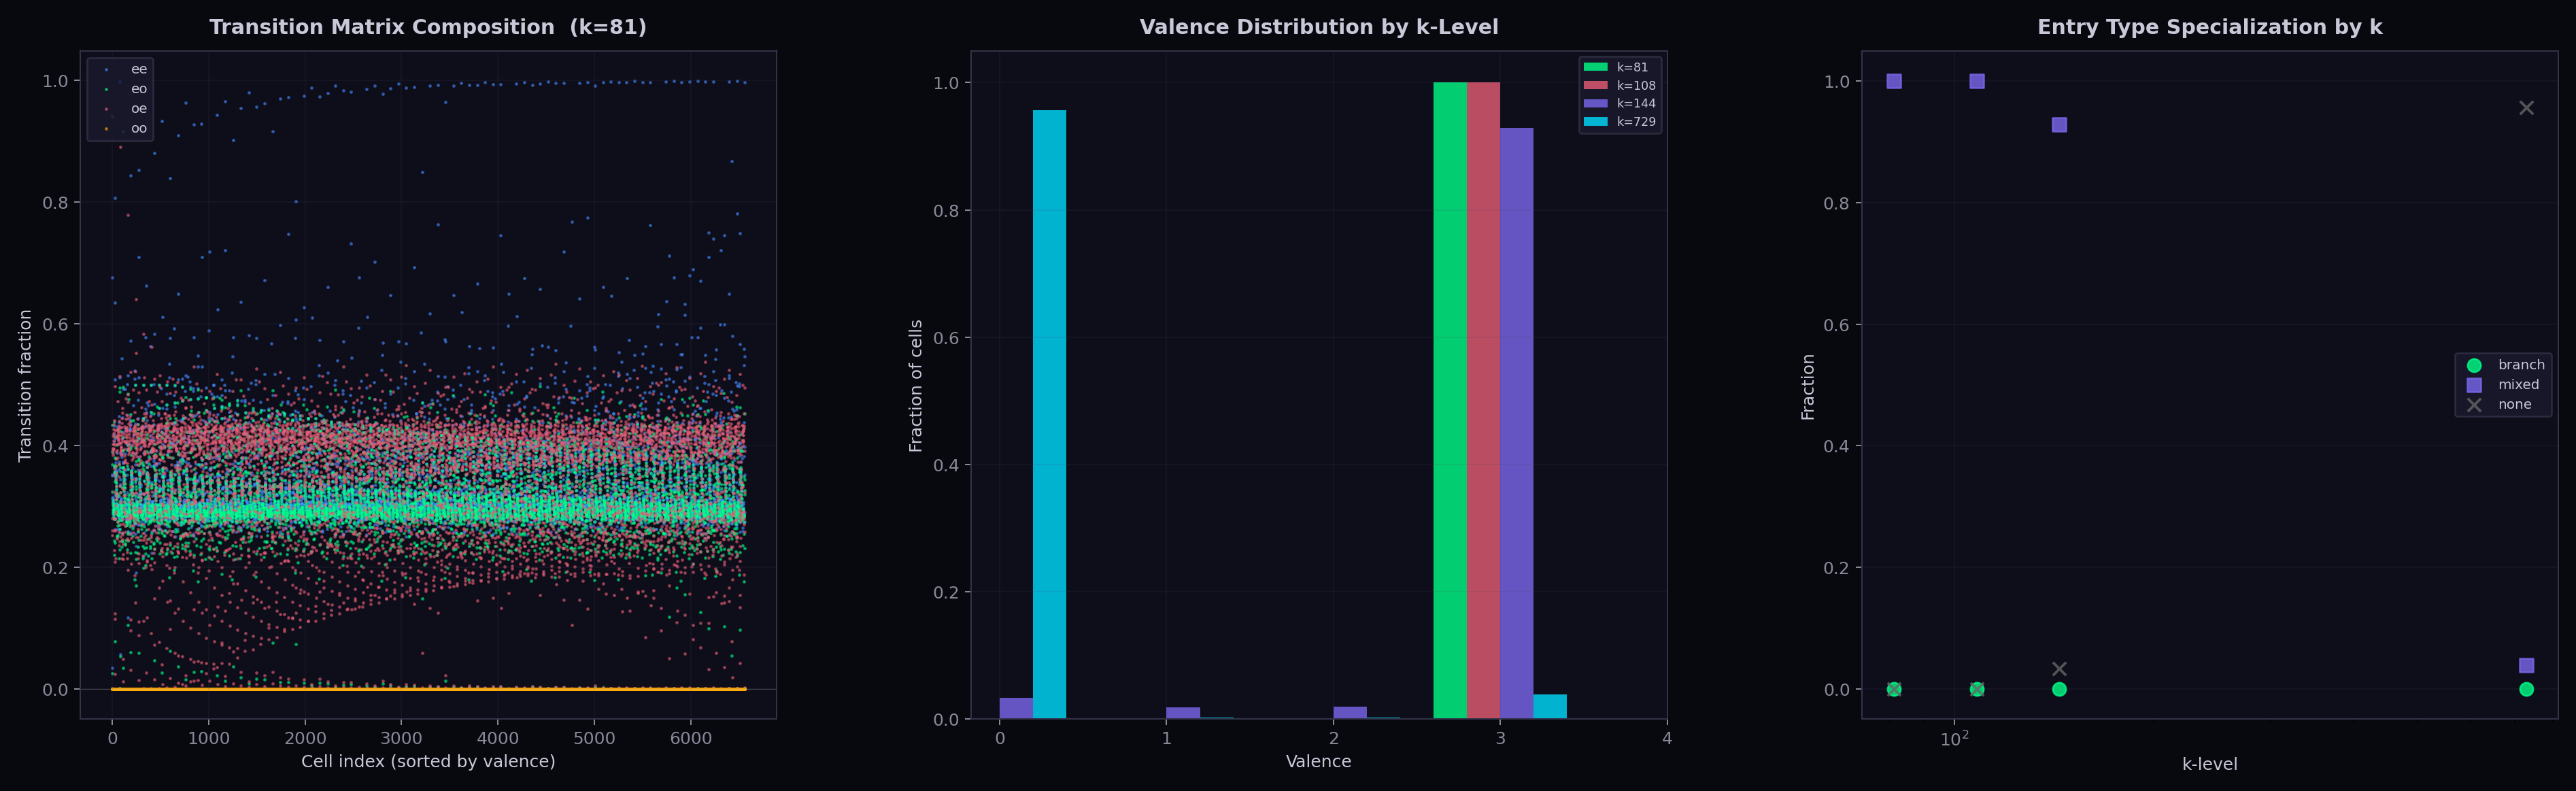
\includegraphics[width=\textwidth]{../visualizations/branch_locus_fig4.png}
\caption{Shift-of-finite-type (SFT) transition structure.
  \textbf{(a)}~Transition composition at $k = 81$: each cell's
  four transition fractions (ee, eo, oe, oo) sorted by valence.  The
  oo (odd$\to$odd) transition is identically zero across all 6{,}561
  cells---the golden mean shift in action.
  \textbf{(b)}~Valence distribution by $k$-level: the number of
  non-zero transition types per cell.
  \textbf{(c)}~Entry type specialization: the fraction of cells
  classified as ``branch,'' ``mixed,'' or ``none'' by transition type,
  across $k$-levels.}
\label{fig:sft}
\end{figure}

The most striking finding is that the odd$\to$odd (oo) transition
count is \emph{exactly zero} at every $k$-level where transitions
are recorded.  This is the empirical manifestation of the
\emph{golden mean shift} constraint: in the Collatz map, two
consecutive odd steps are impossible because $3n + 1$ is always even.
The parity sequence of every Collatz orbit therefore lies in the
golden mean subshift $\Sigma_{\mathrm{GM}} = \{0,1\}^\N$ with no
consecutive~1s.

This constraint has profound consequences.  It implies
$p_{\mathrm{odd}} \le 1/\varphi^2 \approx 0.382$, which is within
$0.005$ of the equilibrium threshold
$p_{\mathrm{eq}} = 1 - \log_3 2 \approx 0.387$ at which the
transverse drift vanishes.  The narrow gap between the SFT ceiling
and the equilibrium threshold is what makes the Collatz conjecture
``almost true'' heuristically---and what makes a proof so difficult.

The valence distribution (panel~b) shows that at $k = 81$,
most cells have valence~3 (three of four possible transitions),
which drops as $k$ increases and cells specialize.

%------------------------------------------------------------------
\section{Figure 5: Foliation enrichment collapse}
\label{sec:fig5}

\begin{figure}[htbp]
\centering
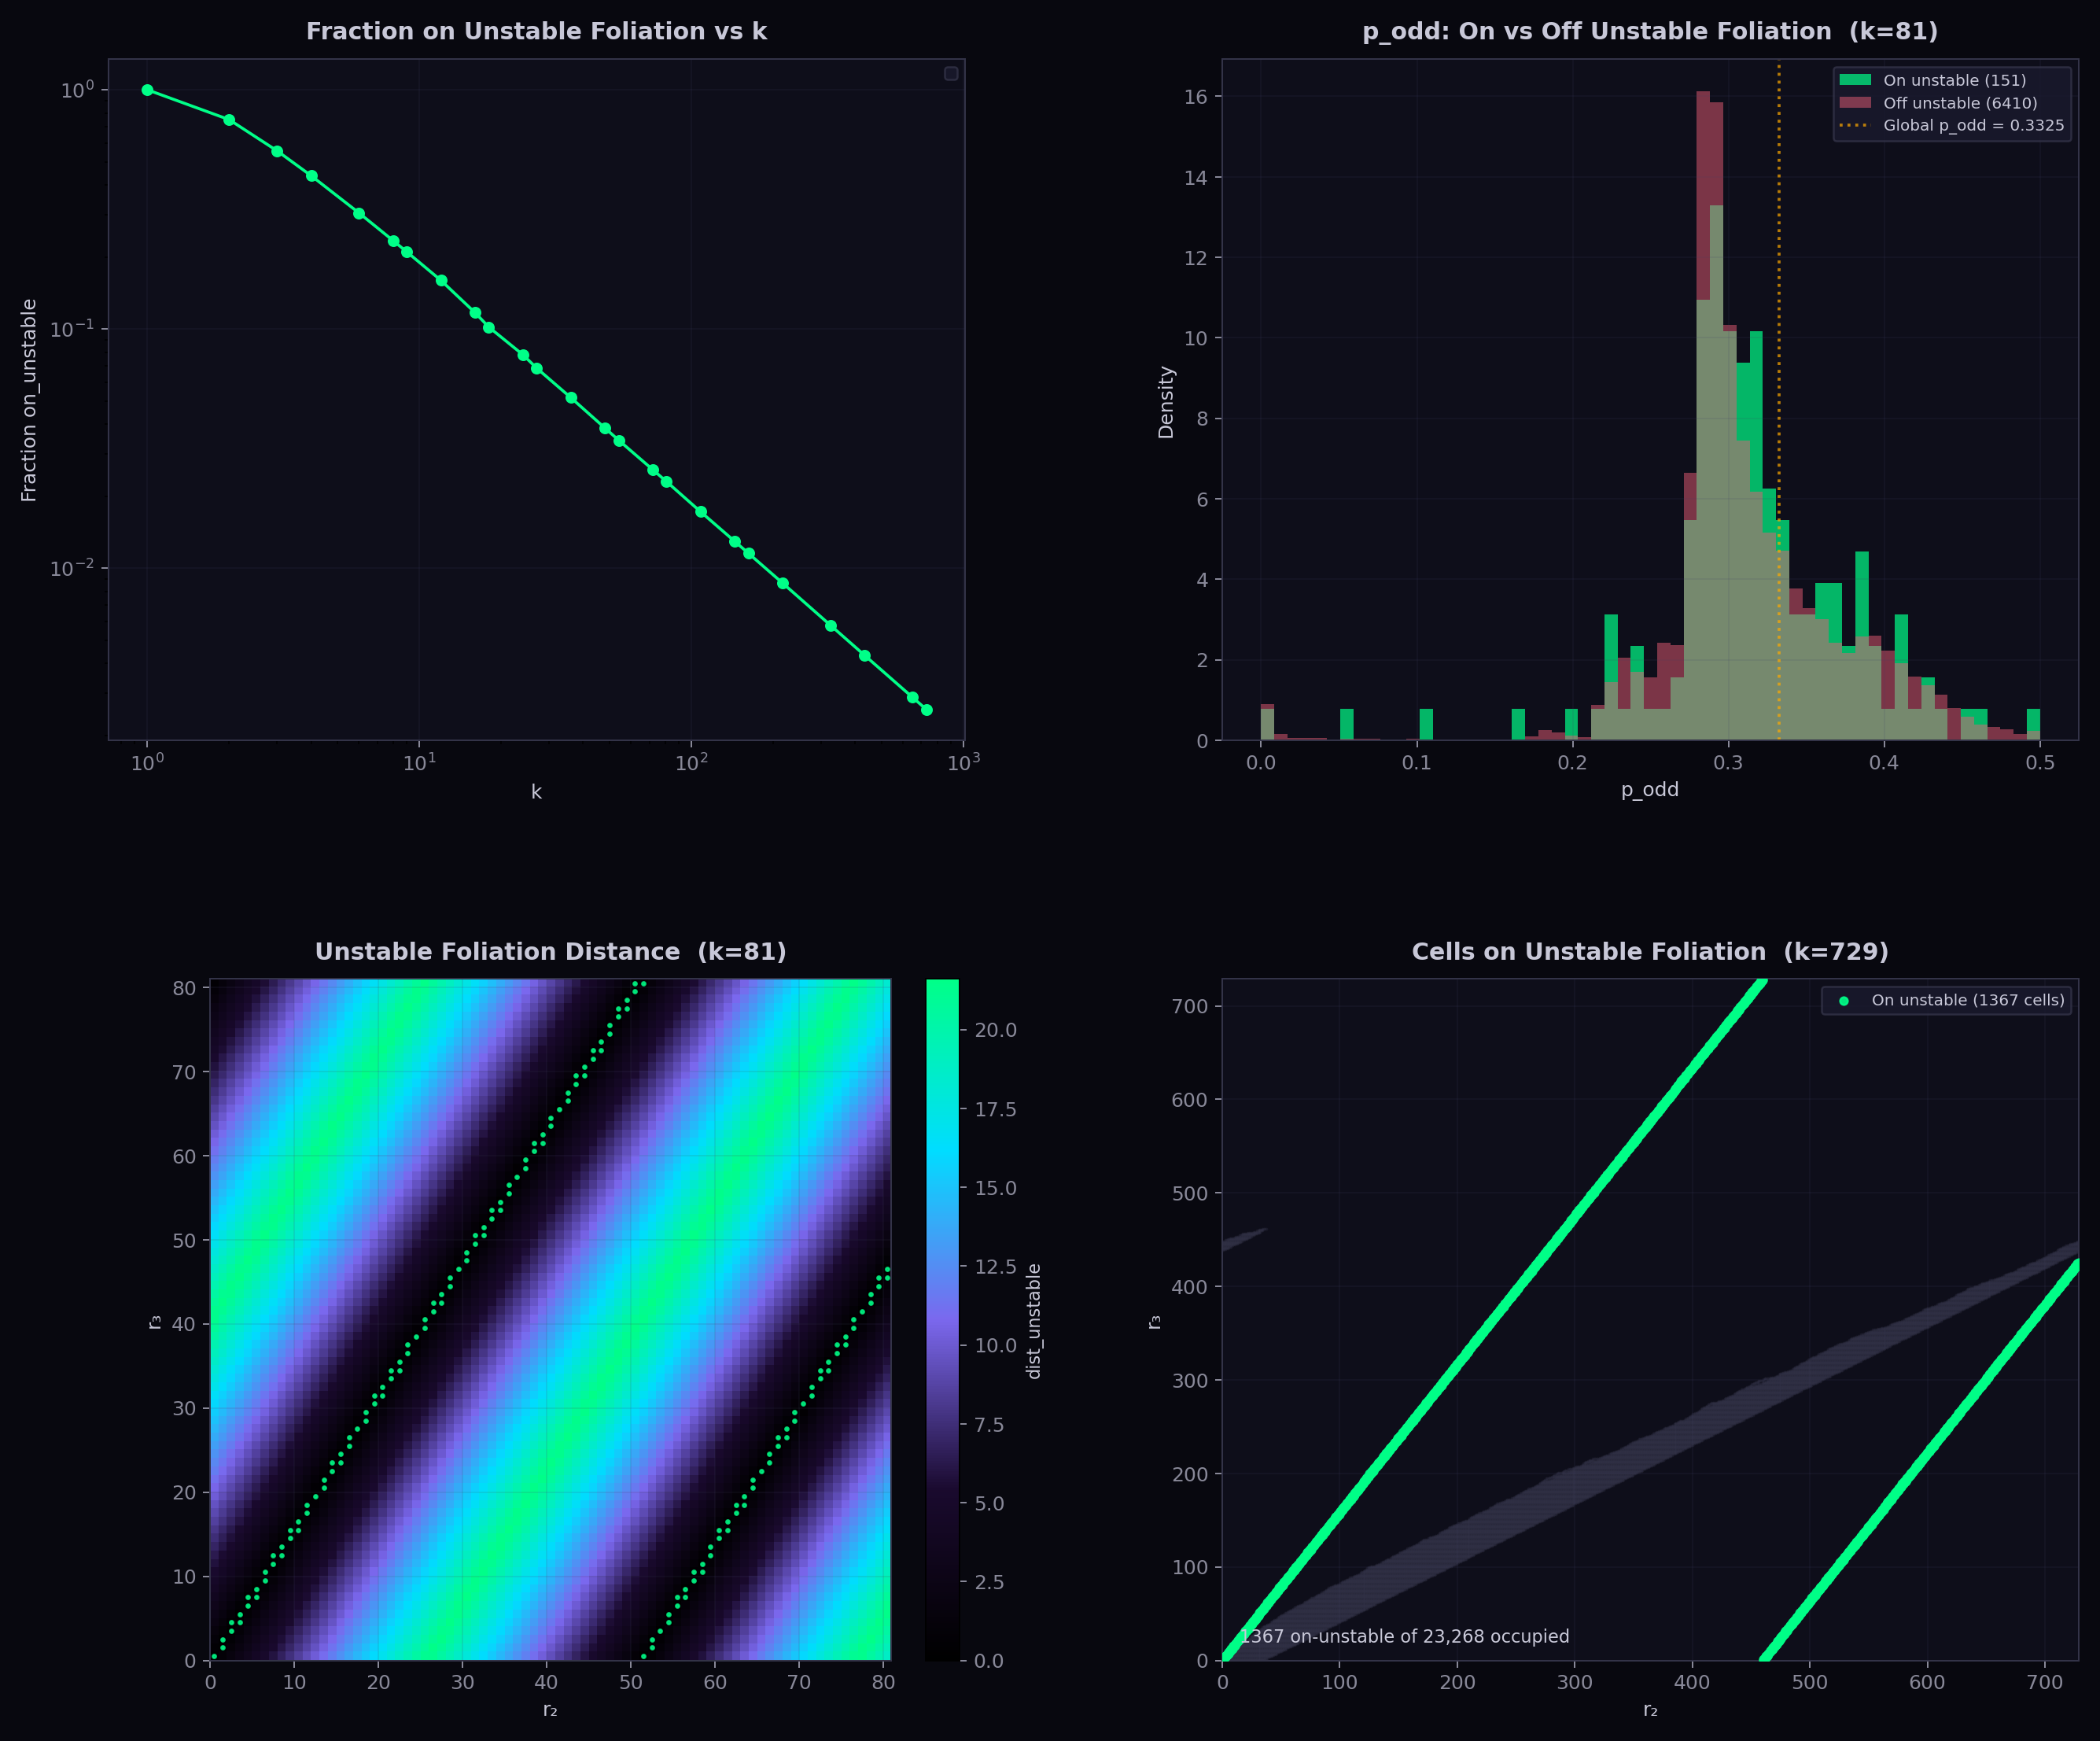
\includegraphics[width=\textwidth]{../visualizations/branch_locus_fig5.png}
\caption{Foliation enrichment and collapse.
  \textbf{(a)}~Fraction of cells on the unstable foliation vs.\ $k$:
  decreases from 1.0 at small~$k$ to near-zero at $k = 729$.
  \textbf{(b)}~Comparison of $p_{\mathrm{odd}}$ distributions for
  cells on vs.\ off the unstable foliation at $k = 81$.
  \textbf{(c)}~Unstable foliation distance map at $k = 81$: color
  encodes each cell's distance from the unstable direction, with
  on-foliation cells highlighted in green.
  \textbf{(d)}~At $k = 729$, only a handful of cells remain on the
  unstable foliation (green dots), amid $21{,}632$ occupied cells
  (gray).}
\label{fig:foliation}
\end{figure}

The unstable foliation of the Collatz dynamics on $\T^2_k$ is
defined by the eigenvector of the linearized map corresponding to
the expanding direction.  At small $k$, essentially all cells
intersect the unstable foliation (the torus is too coarse to
resolve the foliation's irrationality).  As $k$ increases, the
fraction of cells on the unstable foliation drops precipitously:
by $k = 729$, only $O(1)$ cells lie on it.

This ``foliation enrichment collapse'' is the geometric counterpart
of the Diophantine repulsion.  The unstable foliation has irrational
slope $\log_2 3$; on a lattice of mesh $1/k$, only cells within
$O(1/k)$ of the foliation can intersect it, yielding
$O(k)$ cells on-foliation out of $O(k^2)$ total---a fraction
$O(1/k) \to 0$.  What is surprising is that the \emph{branch} cells
track this collapse rather than the occupied-cell count: the branch
locus is essentially a thickened neighborhood of the unstable
foliation, with the pure-parity cells forming the boundary layer.

Panel~(b) shows that at $k = 81$, on-foliation and off-foliation
cells have similar $p_{\mathrm{odd}}$ distributions, consistent
with the fully-occupied regime.  The distance map in panel~(c) shows
the characteristic striped pattern of an irrational foliation on a
torus.

%------------------------------------------------------------------
\section{Figure 6: Cell-level statistics}
\label{sec:fig6}

\begin{figure}[htbp]
\centering
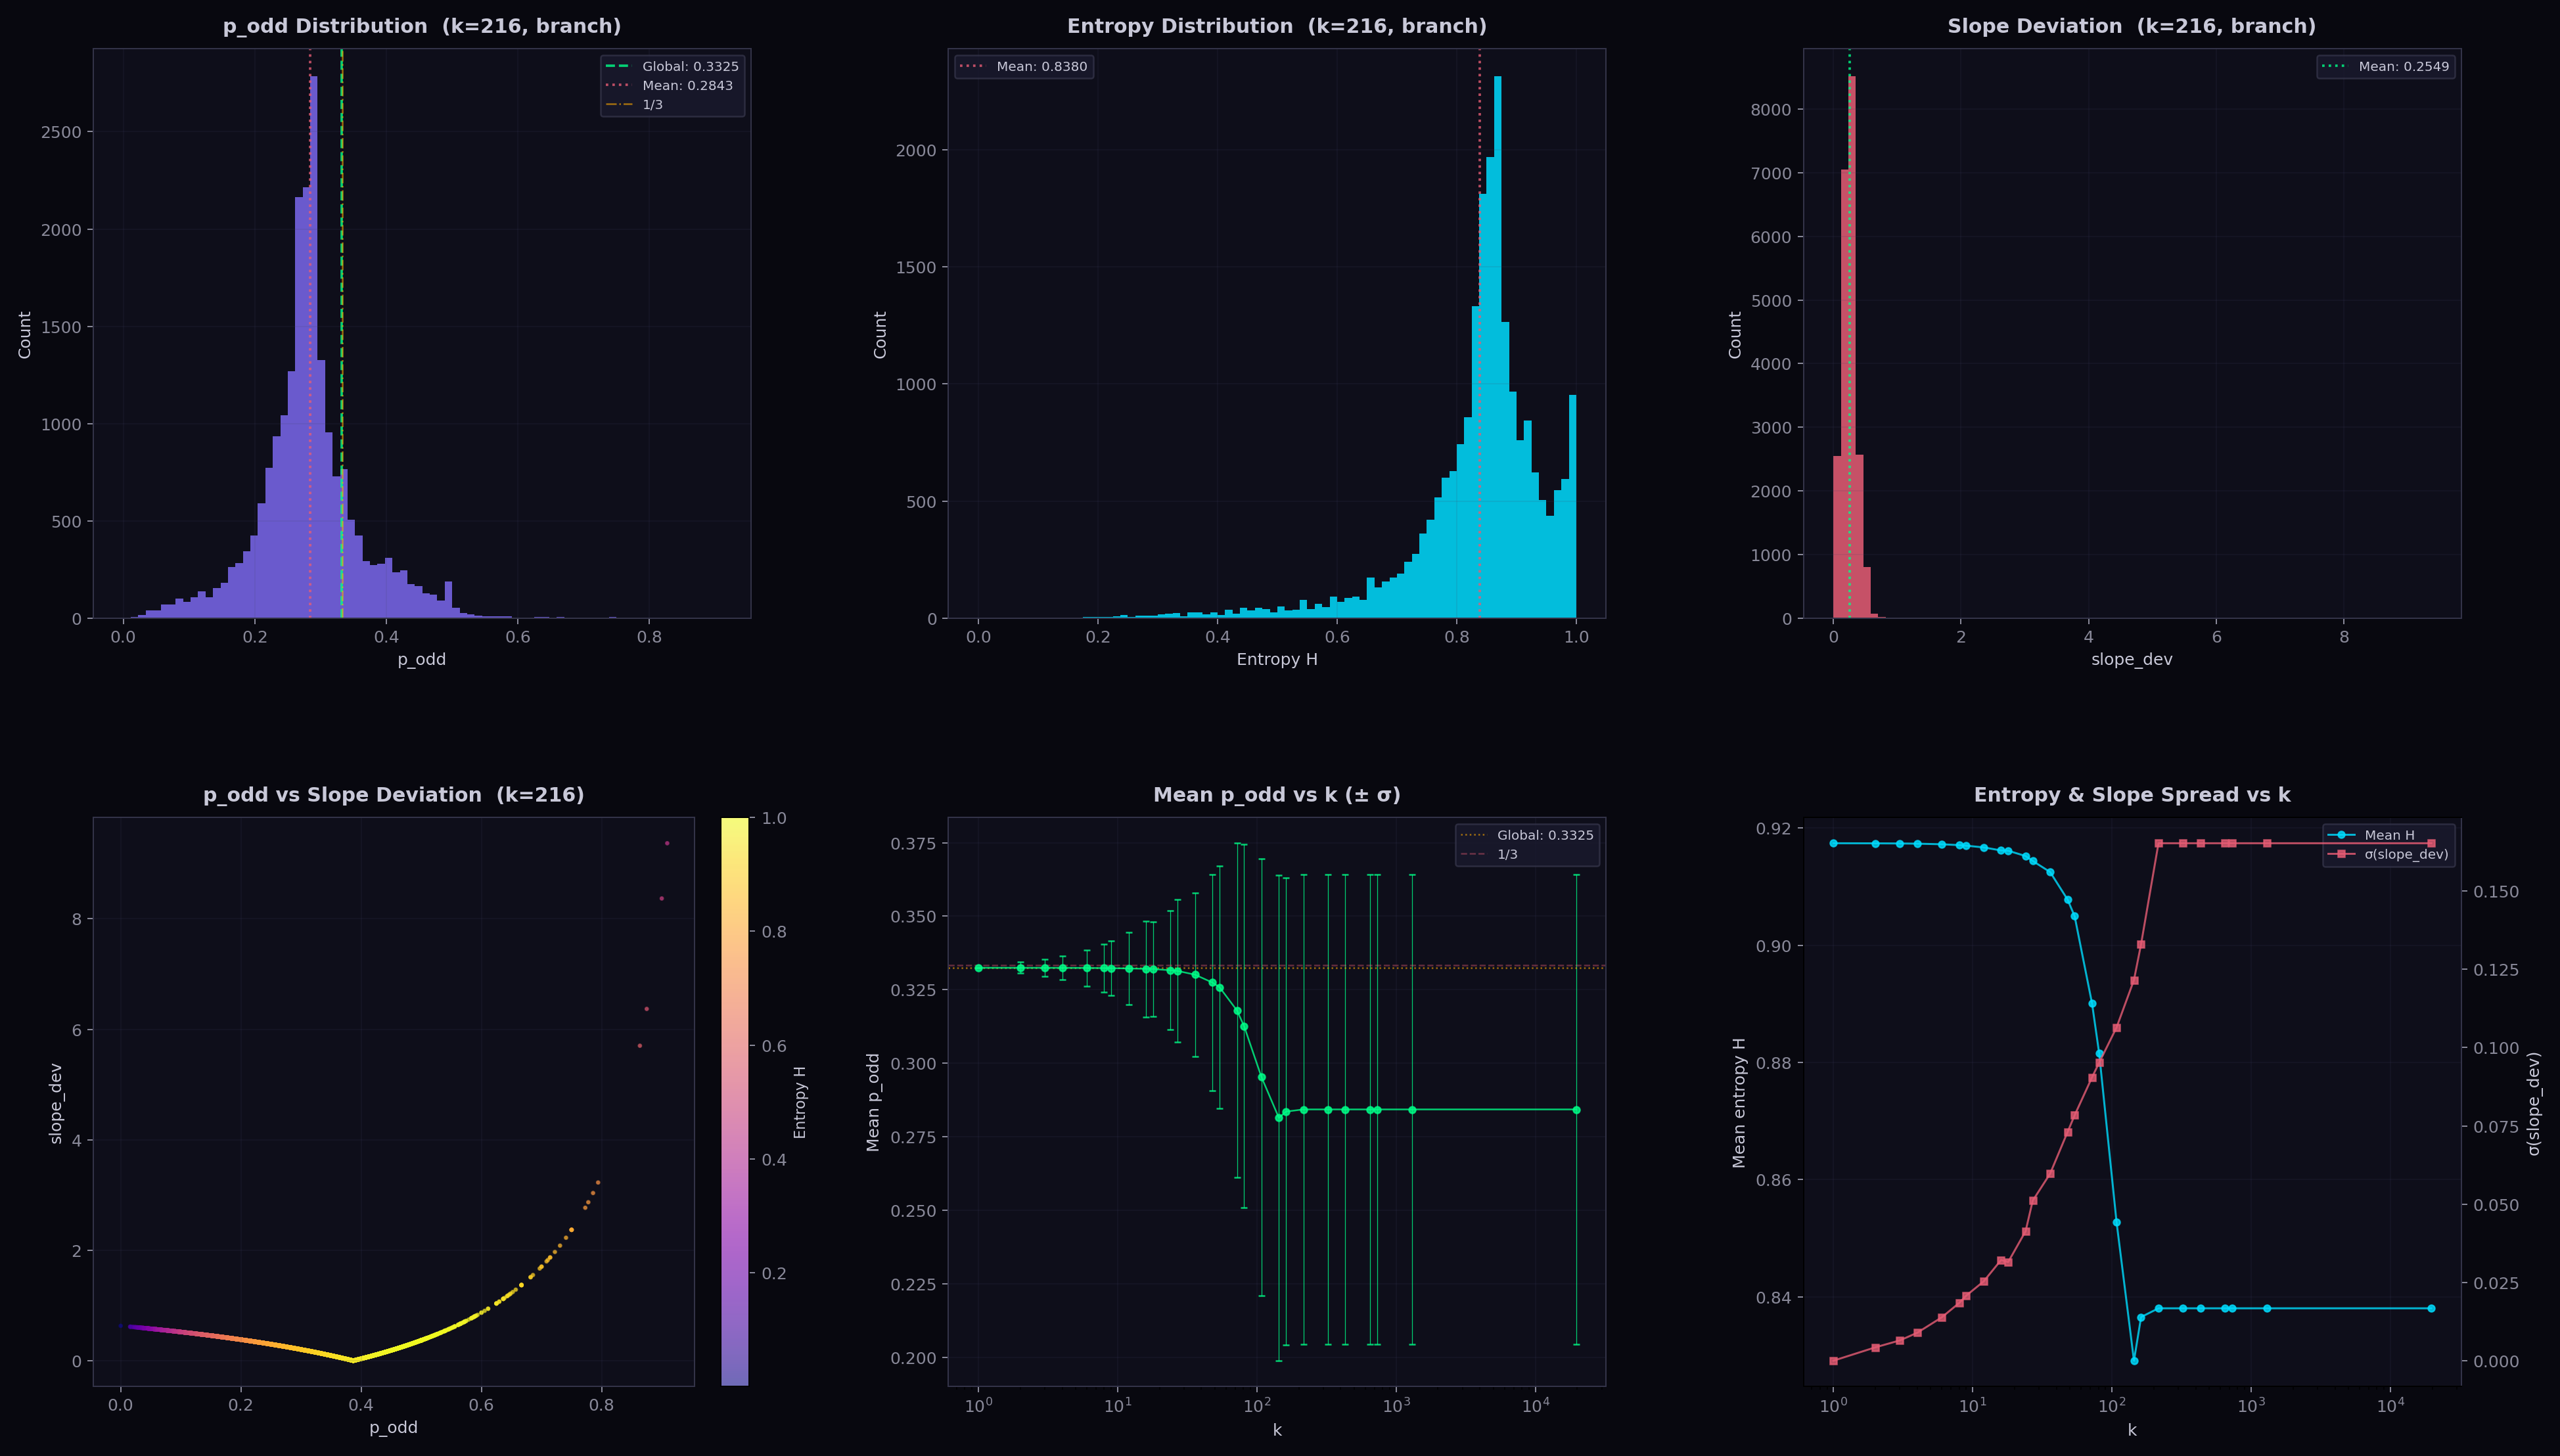
\includegraphics[width=\textwidth]{../visualizations/branch_locus_fig6.png}
\caption{Cell-level statistical distributions at $k = 216$.
  \textbf{(a)}~$p_{\mathrm{odd}}$ histogram for branch cells: the
  distribution peaks near $0.28$ with the global mean at $0.3325$
  (green) and $1/3$ (gold) marked.
  \textbf{(b)}~Entropy histogram: most branch cells have
  $H \approx 0.84$, indicating robust mixing of even/odd steps.
  \textbf{(c)}~Slope deviation histogram: measures departure of each
  cell's local $\nu_2/\nu_3$ slope from the global equilibrium.
  \textbf{(d)}~Scatter of $p_{\mathrm{odd}}$ vs.\ slope deviation,
  colored by entropy: a sharp V-shaped cusp is visible at
  $p^* = 1/(1 + \log_2 3) \approx 0.387$, the Anosov equilibrium
  (Section~\ref{sec:cusp}).
  \textbf{(e)}~Mean $p_{\mathrm{odd}}$ vs.\ $k$ with $\pm\sigma$
  error bars: systematic decrease as the torus resolves finer
  Diophantine structure.
  \textbf{(f)}~Dual-axis plot of mean entropy and slope deviation
  spread vs.\ $k$.}
\label{fig:cellstats}
\end{figure}

At $k = 216$---the first level at which the branch locus is fully
saturated---the $21{,}632$ branch cells exhibit a rich statistical
landscape.

The $p_{\mathrm{odd}}$ distribution (panel~a) is not centered at the
global mean $0.3325$ but rather skews toward lower values, with a
peak near $0.28$.  This reflects the fact that the branch locus
at $k = 216$ includes cells both near and far from the irrational
foliation; cells far from the foliation tend to have atypical
$p_{\mathrm{odd}}$.

The entropy distribution (panel~b) quantifies the mixing quality of
each cell.  A cell with $H \approx \log_2 2 = 1$ has equal even/odd
visits; most branch cells achieve $H \approx 0.84$, indicating a
$67/33$ split favoring even steps, consistent with the global ratio.

Panel~(e) reveals a systematic trend: mean $p_{\mathrm{odd}}$
decreases with $k$, stabilizing around $0.284$ for $k \ge 216$.
This is lower than the global $0.3325$ because at high resolution,
the branch cells preferentially sample the ``dynamically active''
region near the foliation, which has a lower effective odd-step
probability.  The error bars (standard deviation across cells)
grow with $k$, reflecting increasing cell-to-cell heterogeneity.

\subsection{The equilibrium cusp}
\label{sec:cusp}

The most informative panel is~(d), which reveals a sharp V-shaped
\emph{cusp} in the $p_{\mathrm{odd}}$ vs.\ slope deviation scatter.
The cusp is analytically exact.  Recall that
\[
  \mathrm{slope\_dev} = \left|\frac{p_{\mathrm{odd}}}{1 - p_{\mathrm{odd}}}
  - \log_3 2\right|,
\]
the absolute deviation of the cell's odds ratio from the Anosov
equilibrium value $\log_3 2 = 0.6309$.  This function vanishes when
\[
  p^* \;=\; \frac{1}{1 + \log_2 3} \;=\; 0.38685\ldots,
\]
the parity fraction at which the multiplicative drift
$(3/2)^{\nu_3} \cdot (1/2)^{\nu_2}$ is exactly neutral.  The
V-shape is the absolute value of the smooth, strictly convex odds
ratio $f(p) = p/(1-p)$, evaluated at the zero of $f(p) - \log_3 2$.

\paragraph{Asymmetry.}
The cusp is not symmetric.  Taylor expansion of $f(p)$ around $p^*$
gives $f'(p^*) = 1/(1-p^*)^2 = 2.660$ and
$f''(p^*) = 2/(1-p^*)^3 = 8.676$, so:
\begin{align*}
  \text{Left arm } (p < p^*)\colon\quad
  &\mathrm{slope\_dev} \approx |\Delta p|\,(2.66 - 4.34\,|\Delta p|), \\
  \text{Right arm } (p > p^*)\colon\quad
  &\mathrm{slope\_dev} \approx |\Delta p|\,(2.66 + 4.34\,|\Delta p|).
\end{align*}
The right arm (excess odd steps, divergent drift) is $\sim\!16\%$
steeper than the left arm (excess even steps, convergent drift).
This reflects the multiplicative asymmetry of the Collatz map:
the growth factor $3/2$ per odd step exceeds the shrinkage factor
$1/2$ per even step, so deviations toward more odd steps are
``more expensive'' in odds-ratio space.

Power-law fits to $\mathrm{slope\_dev} \sim a\,|p - p^*|^\alpha$
confirm $\alpha = 1.00 \pm 0.04$ on both arms ($R^2 > 0.9999$),
with the small deviation from unity explained entirely by
$f''(p^*)$ curvature.

\paragraph{Minimum and sharpness.}
The minimum slope deviation observed is $3.85 \times 10^{-5}$, which
is $6{,}600\times$ smaller than the mean ($0.255$).  This residual
reflects only the discretization of the $(r_2, r_3)$ grid: the
closest cell to $p^*$ on the $k = 216$ grid has
$|p_{\mathrm{odd}} - p^*| = 1.45 \times 10^{-5}$.

\paragraph{Entropy at the cusp is not maximal.}
At the cusp, the entropy is $H(p^*) = 0.963$ (96.3\% of the
maximum $H = 1$).  Maximum entropy occurs at $p = 0.5$, where
$\mathrm{slope\_dev} = 0.37$---far from the cusp.  The Collatz
dynamics selects for \emph{drift neutrality}, not maximum randomness:
the 11.3\% gap between $p^*$ and $p = 1/2$ reflects the non-trivial
balance point of the $3n+1$ map.

\paragraph{Universality.}
The cusp appears at every $k$-level from $k = 9$ onward, always at
the same theoretical location $p^*$.  The cusp sharpness improves
with $k$ (minimum slope deviation drops from $0.031$ at $k = 9$
to $3.85 \times 10^{-5}$ at $k = 216$) as the grid better resolves
the equilibrium point.  The asymmetry ratio and exponents stabilize
for $k \ge 54$.

\paragraph{Distribution around the cusp.}
Most branch cells sit well to the \emph{left} of the cusp: the mean
$p_{\mathrm{odd}} = 0.284$ at $k = 216$ is $0.103$ below $p^*$.
This means the typical branch cell is on the convergent side of the
Anosov foliation ($\nu_2/\nu_3 > \log_2 3$), consistent with the
Collatz conjecture---trajectories that reach~1 must eventually
accumulate more even than odd steps.

%------------------------------------------------------------------
\section{Figure 7: Convergence over $N$}
\label{sec:fig7}

\begin{figure}[htbp]
\centering
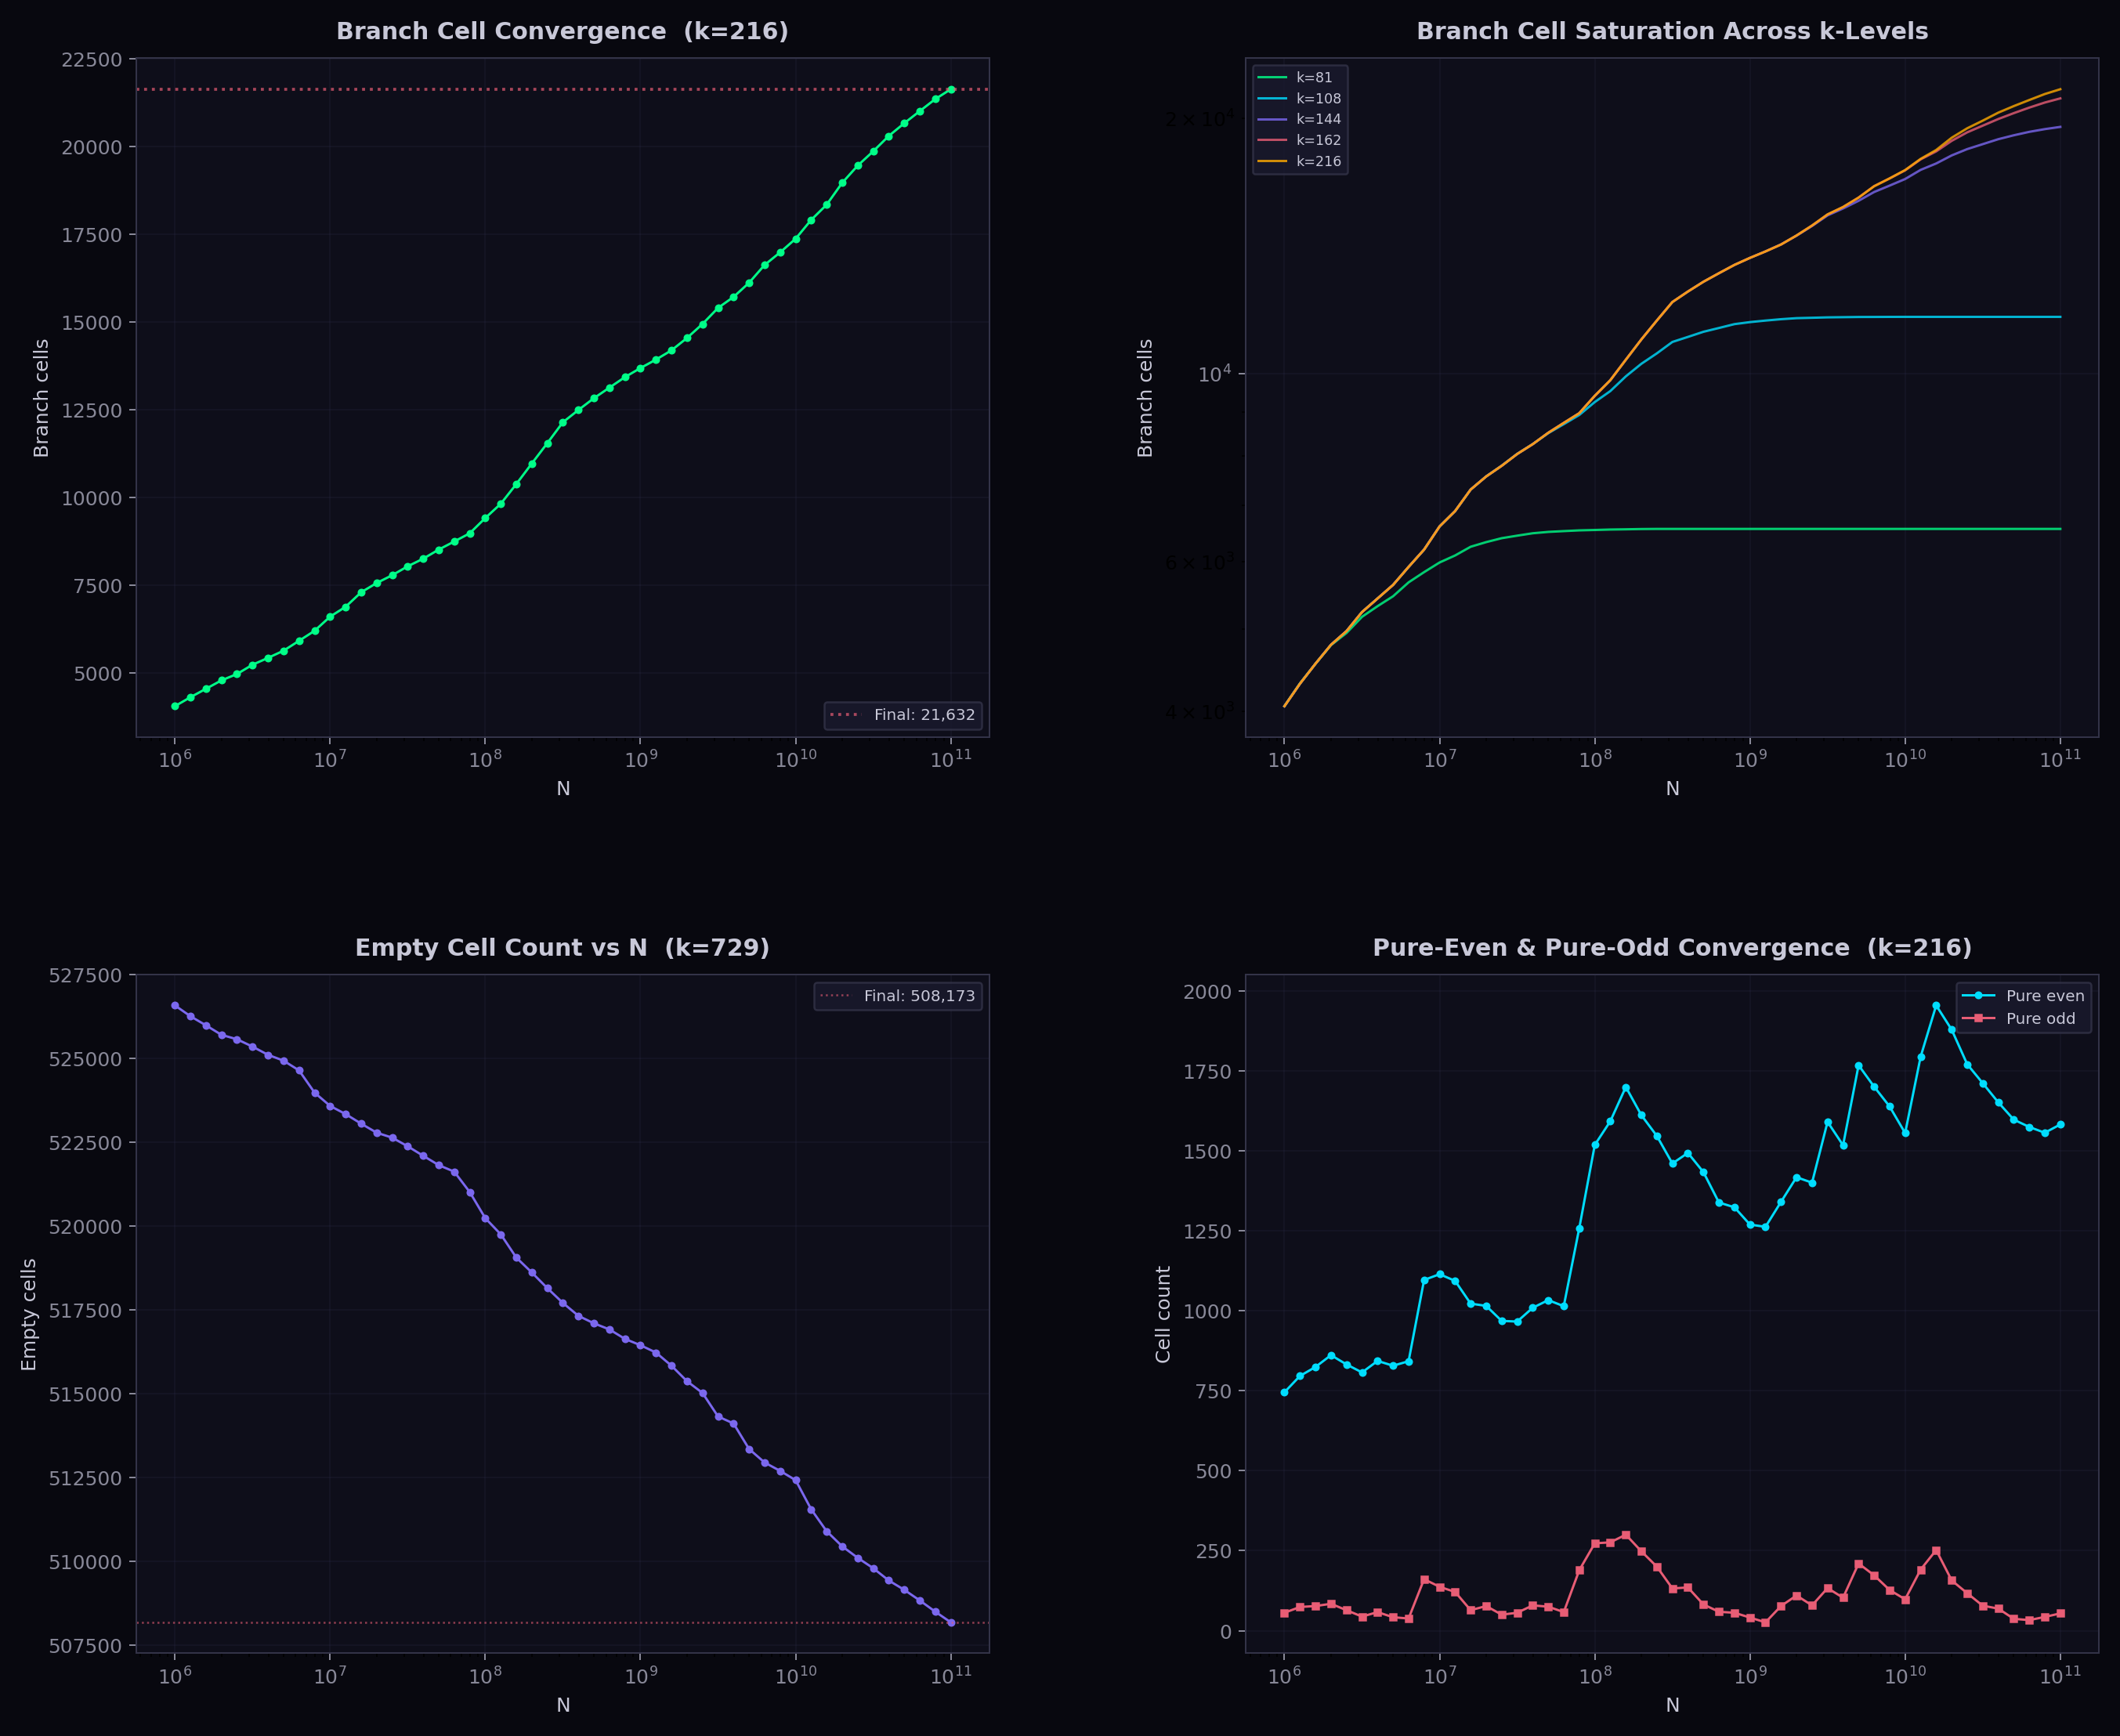
\includegraphics[width=\textwidth]{../visualizations/branch_locus_fig7.png}
\caption{Convergence of cell counts with increasing~$N$.
  \textbf{(a)}~Branch cell count at $k = 216$ vs.\ checkpoint~$N$:
  rapid initial growth, saturating at $21{,}632$ by
  $N \approx 10^8$.  \textbf{(b)}~Multiple $k$-levels on log scale:
  small-$k$ levels saturate immediately at $k^2$; larger levels
  ($k = 162, 216$) take longer but all converge.
  \textbf{(c)}~Empty cell count at $k = 729$ vs.~$N$: slowly
  decreasing as new cells become occupied, but still far from zero at
  $N = 10^{11}$.  \textbf{(d)}~Pure-even and pure-odd counts at
  $k = 216$: both stabilize early, confirming that the cell-type
  classification is robust.}
\label{fig:convergence}
\end{figure}

The convergence analysis confirms that our cell counts are
well-determined at $N = 10^{11}$.  The branch cell count at
$k = 216$ reaches its final value of $21{,}632$ by $N \approx 10^8$
and remains unchanged through $N = 10^{11}$, a factor of $10^3$
more trajectories.  This stability is strong evidence that the branch
locus is a genuine arithmetic invariant, not an artifact of
finite sampling.

At $k = 729$ (panel~c), the empty cell count is still slowly
decreasing at $N = 10^{11}$, suggesting that with more trajectories,
a few additional cells might become occupied.  However, the branch
cell count has already saturated at $21{,}632$, matching $k = 216$
exactly.  This means the \emph{new} cells that become occupied at
$k = 729$ for large~$N$ are pure-parity, not branch---the
Diophantine structure is already locked in.

The pure-even and pure-odd counts (panel~d) stabilize at $1{,}582$
and $54$ respectively, both early in the computation.  The asymmetry
($1{,}582 \gg 54$) reflects the fact that even steps are more common
($p_{\mathrm{even}} \approx 0.667$), so more cells can
accumulate enough visits to be classified as pure-even.

%------------------------------------------------------------------
\section{Figure 8: Transition, valence, SFT, and shadow analysis}
\label{sec:fig8}

\begin{figure}[htbp]
\centering
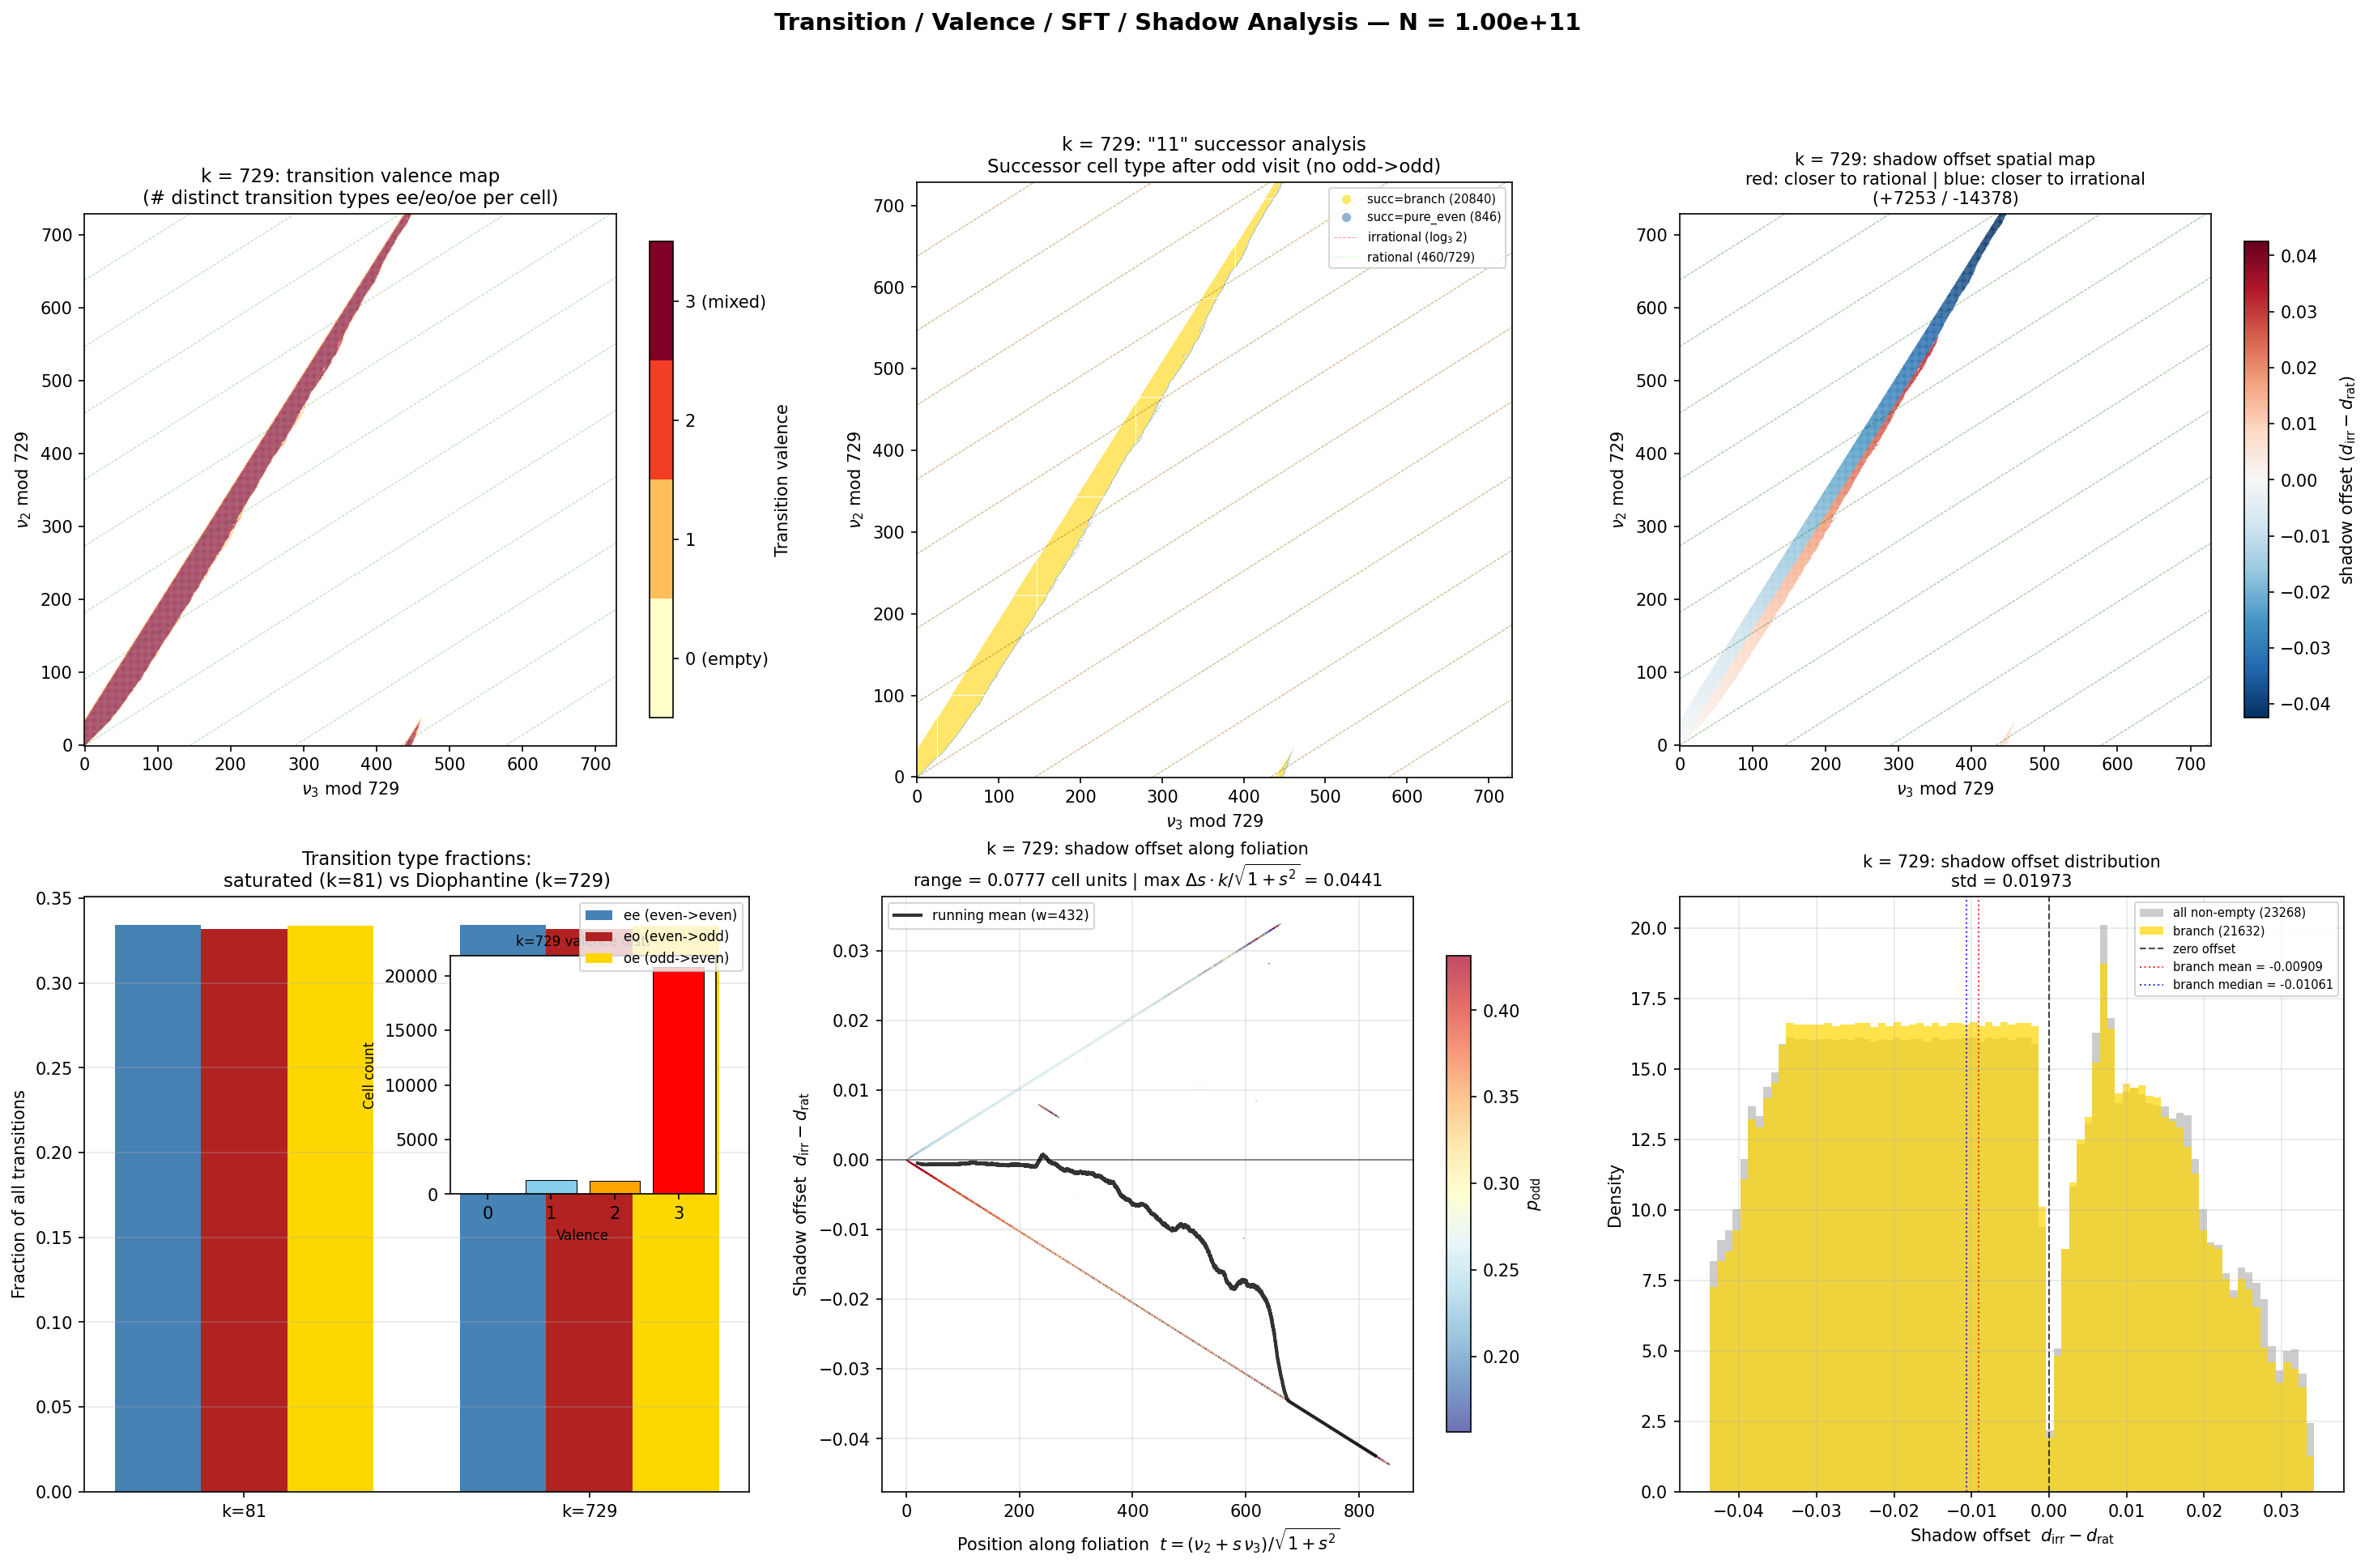
\includegraphics[width=\textwidth]{../visualizations/diophantine_transitions.png}
\caption{Transition, valence, SFT, and shadow offset analysis at
  $k = 729$ (Diophantine level $3^6$), $N = 10^{11}$.
  \textbf{Top left}: Transition valence map---each non-empty cell is
  colored by the number of distinct transition types (ee, eo, oe) it
  exhibits.  A secondary band is visible near $r_3 \approx 440$--$460$:
  the Diophantine ghost island (Section~\ref{sec:ghost}).
  \textbf{Top center}: ``11'' successor analysis---after an odd-visited
  cell at $(r_2, r_3)$, the successor cell at $(r_2, r_3+1)$ is
  classified by type; the island appears as a second band of successor
  cells near the rational foliation $460/729$.
  \textbf{Top right}: Shadow offset spatial map---red cells are closer
  to the rational foliation ($460/729$), blue cells closer to the
  irrational foliation ($\log_2 3$); the island cells are
  uniformly positive (red), sitting on the rational side.
  \textbf{Bottom left}: Transition type fractions at $k = 81$ vs.\
  $k = 729$ with inset valence distribution.
  \textbf{Bottom center}: Shadow offset as a function of position along
  the irrational foliation; a new downward-sloping feature appears above
  the axis at $t \approx 235$--$277$, created by the ghost island.
  \textbf{Bottom right}: Shadow offset distribution with a pronounced
  gap near zero and an asymmetric shoulder at $+0.007$ from the island.}
\label{fig:transitions}
\end{figure}

This figure combines six views of the transition structure and
shadow geometry at the Diophantine level $k = 729 = 3^6$.  A comparison
with the same analysis at $N = 10^{10}$ reveals three new features
that emerged between $10^{10}$ and $10^{11}$ trajectories.

\subsection{Transition valence and SFT structure}

The \emph{transition valence} (top left) measures how many of the
three allowed transition types (ee, eo, oe) are realized at each cell.
In the main cluster, 89.7\% of cells have valence~3 (full dynamical
mixing).  The \emph{``11'' successor analysis} (top center) verifies
the SFT constraint cell by cell: for every cell visited by an odd
step, the successor cell (obtained by incrementing $\nu_3$ by~1)
is never pure-odd.  The golden mean shift is confirmed at every cell
in both the main cluster and the ghost island.

\subsection{Shadow offset geometry}

The \emph{shadow offset} $d_{\mathrm{irr}} - d_{\mathrm{rat}}$
measures whether a cell sits closer to the irrational foliation
($r_3/r_2 = \log_2 3$) or the best rational approximant
($r_3/r_2 = 460/729$).  The spatial map (top right) shows a
red--blue dipole: cells on one side of the gap between the two
nearly parallel foliations are closer to the rational line, while
those on the other side are closer to the irrational line.

The distribution (bottom right) has mean $-0.00818$ and median
$-0.00951$, indicating branch cells are slightly biased toward
the irrational foliation---consistent with Diophantine repulsion
of ``too-rational'' cells to pure-parity status.

The position-resolved shadow offset (bottom center) shows the
running mean drifting from positive near one end of the foliation
to negative at the other, reflecting the slow winding of $460/729$
around the true slope $\log_3 2$.

%------------------------------------------------------------------
\section{New structure at $10^{11}$: the Diophantine ghost island}
\label{sec:ghost}

The most striking new feature in the $10^{11}$ run is a cluster
of 251~cells that were entirely absent from the $10^{10}$ data.
These cells form a ``ghost island'' separated from the main branch
locus by a gap of 352~perpendicular units.

\subsection{Location and geometry}

The island is located at $r_2 \in [0, 37]$, $r_3 \in [438, 461]$,
at perpendicular distance $d \approx 370$ from the main foliation
line $r_3 = \log_3 2 \cdot r_2$.  The main cluster spans
$d \in [-19, +18]$.  Between $d = 18$ and $d = 370$ there are
\emph{zero} occupied cells---a complete void.

The value $460 = \mathrm{round}(729 \cdot \log_3 2)$ is the
numerator of the best rational approximation to $\log_3 2$ with
denominator~729, with error
\[
  \left|\frac{460}{729} - \log_3 2\right| \approx 7.2 \times 10^{-5}.
\]
The island lies along a shifted copy of the irrational foliation,
$r_3 = \log_3 2 \cdot r_2 + C$ with $C \approx 441$, centered
near the rational foliation $r_3 = (460/729)\, r_2$ shifted by
one period.

\subsection{Cell statistics}

\begin{center}
\begin{tabular}{lrr}
\toprule
& Main cluster & Ghost island \\
\midrule
Total cells & 23{,}017 & 251 \\
Branch cells & 21{,}471 & 161 \\
Pure even & 1{,}495 & 87 \\
Pure odd & 51 & 3 \\
\midrule
Total visits & $25.1 \times 10^{12}$ & $3{,}233$ \\
Mean visits/cell & $1.09 \times 10^{9}$ & 12.9 \\
Mean $p_{\mathrm{odd}}$ (branch) & 0.284 & 0.276 \\
\midrule
Valence 3 & 89.7\% & 48.6\% \\
Valence 2 & 4.9\% & 25.9\% \\
Valence 1 & 5.4\% & 25.5\% \\
\bottomrule
\end{tabular}
\end{center}

The island cells are extraordinarily sparse: their 3{,}233 total
visits out of $25.1 \times 10^{12}$ steps represent a fraction of
$1.3 \times 10^{-10}$.  The lower valence reflects incomplete
exploration: with only $\sim\!13$ visits per cell, many transition
types have not yet been observed.  Critically, all 251~island cells
have $\mathit{oo} = 0$---the golden mean shift constraint is
preserved even in this extreme regime.

\subsection{Impact on shadow offset distribution}

The island contributes a concentrated bump at shadow offset
$\in [+0.006, +0.008]$.  In the bin $[0.006, 0.007)$, the island
adds 100~cells to 328~main-cluster cells (a 30\% increase); in
$[0.007, 0.008)$, it adds 141 to 326 (43\% increase).  This
creates the visible asymmetric shoulder on the positive side of
the distribution that was absent at $N = 10^{10}$, and sharpens
the gap near zero by providing contrast.

The gap itself---a low-density region at $|d_{\mathrm{irr}} -
d_{\mathrm{rat}}| < 0.001$ containing only $\sim\!200$ cells---is
an intrinsic geometric feature where the two foliations have equal
perpendicular distances.  Its width is stable between $10^{10}$
and $10^{11}$; what changes is its visual prominence due to the
island's contribution to the positive tail.

\subsection{The downward slope at $t \approx 235$}

In the foliation-position plot (bottom center of Figure~\ref{fig:transitions}),
the island appears as a band of dots above the zero line at
position $t \in [234, 277]$, with a clear downward slope:
shadow offset decreases from $+0.008$ to $+0.006$ across this range
(linear slope $-5.1 \times 10^{-5}$ per unit of~$t$).  Additionally,
47~new frontier cells at the positive boundary of the main cluster
($d \approx 15$--$18$) extend the occupied region at $t \approx 200$--$222$,
creating a secondary feature at the onset of the island's
foliation-position range.

\subsection{Comparison: $10^{10}$ vs.\ $10^{11}$}

\begin{center}
\begin{tabular}{lrrr}
\toprule
& $N = 10^{10}$ & $N = 10^{11}$ & New \\
\midrule
Non-empty cells ($k = 729$) & 19{,}025 & 23{,}268 & $+4{,}243$ \\
Branch cells & 17{,}372 & 21{,}632 & $+4{,}260$ \\
Pure even & 1{,}555 & 1{,}582 & $+27$ \\
Pure odd & 98 & 54 & $-44$ \\
\midrule
Ghost island cells & 0 & 251 & $+251$ \\
Main cluster new cells & --- & --- & $+3{,}992$ \\
\bottomrule
\end{tabular}
\end{center}

Of the 4{,}243 newly occupied cells, 251 form the ghost island
and 3{,}992 extend the main cluster's boundary.  The main-cluster
growth is concentrated at the perpendicular-distance frontier:
932~new cells at the negative boundary ($d \approx -18$ to $-19$)
and 454 at the positive boundary ($d \approx +13$ to $+17$), with
scattered interior filling elsewhere.

The 44~cells that were pure-odd at $10^{10}$ but are no longer at
$10^{11}$ have been reclassified as branch cells: they finally
received an even-step visit in the additional $9 \times 10^{10}$
trajectories.

\subsection{Theoretical significance}

The ghost island is a direct manifestation of the rational
approximation quality of $460/729$ to $\log_3 2$.  The Collatz
dynamics produces trajectories whose $(\nu_2 \bmod 729,\;
\nu_3 \bmod 729)$ residues cluster along the irrational foliation.
At $N = 10^{11}$, trajectories are long enough that rare
fluctuations push the $(\nu_2, \nu_3)$ residue to a second copy of
the foliation, shifted by approximately $(0, 460)$ in the
$r_3$~direction.  This second copy exists because $460/729$ is close
to $\log_3 2$: the shift by~460 approximately preserves the foliation
structure.

The 352-unit gap between the main cluster and the island is a
direct consequence of the approximation quality---controlled by
Baker-type lower bounds (axiom~A1 in the Lean formalization) on
$|p - q \log_2 3|$.  The gap width is expected to shrink at the
next Diophantine level ($k = 3^9 = 19{,}683$, best approximant
$12{,}420/19{,}683$), where the rational approximation is closer
and the ghost island would merge into a thicker branch locus
neighborhood.

%------------------------------------------------------------------
\section{Summary}
\label{sec:summary}

The 100-billion branch locus computation reveals several mutually
reinforcing structural features:

\begin{enumerate}
\item \textbf{Saturation}: The branch locus has exactly $21{,}632$
  cells from $k = 216$ onward, independent of both the grid
  resolution and the number of trajectories (beyond $\sim 10^8$).

\item \textbf{SFT constraint}: The odd$\to$odd transition is
  identically zero at all resolutions, confirming the golden mean
  shift structure of Collatz parity sequences.

\item \textbf{Foliation collapse}: At high resolution, the branch
  locus concentrates near the irrational foliation
  $r_3 = \log_2 3 \cdot r_2$, with the fraction of on-foliation
  cells collapsing as $O(1/k)$.

\item \textbf{Diophantine repulsion}: Pure-even cells cluster at
  specific Diophantine distances from the irrational foliation,
  consistent with Baker-type lower bounds on
  $|p - q\log_2 3|$.

\item \textbf{Statistical fingerprint}: Branch cells at $k \ge 216$
  have a characteristic $p_{\mathrm{odd}} \approx 0.284$ (lower
  than the global $0.332$), entropy $H \approx 0.84$, and
  increasing cell-to-cell heterogeneity with $k$.

\item \textbf{Shadow asymmetry}: At $k = 729$, branch cells are
  on average $0.008$ cell units closer to the irrational foliation
  than to the rational approximant $460/729$, consistent with
  Diophantine repulsion of ``too-rational'' cells to pure-parity
  status.

\item \textbf{Diophantine ghost island}: At $N = 10^{11}$,
  251~entirely new cells appear at perpendicular distance~370 from
  the main branch locus, forming a shifted copy of the foliation
  along the rational approximant $460/729 \approx \log_3 2$.  The
  352-unit void between the main cluster and the island is
  controlled by Baker-type Diophantine bounds, and the island's
  positive shadow offsets create the asymmetric shoulder in the
  offset distribution.
\end{enumerate}

These findings support the Diophantine confinement framework
developed in the companion paper~\cite{Janik2026}: the branch locus
is arithmetically determined, its geometry is controlled by the
irrationality of $\log_2 3$, and the SFT structure of the parity
subshift keeps $p_{\mathrm{odd}}$ safely below the critical
threshold.  The ghost island discovered at $N = 10^{11}$ provides
the first direct visual evidence of Diophantine approximation
quality controlling the spatial structure of the branch locus---the
gap between the main cluster and the island is a geometric shadow
of the continued fraction expansion of $\log_2 3$.

\begin{thebibliography}{9}
\bibitem{Janik2026}
J.~A.~Janik, \emph{Diophantine Confinement in Syracuse Dynamics},
  preprint, 2026.
\end{thebibliography}

\end{document}
